% ---------------------------------------------------------------
% ---------------------------------------------------------------
% This template was developed for the working paper series of
% the Interdisciplinary Laboratory of Computational Social Science (iLCSS)
% at the University of Maryland, College Park

% The template was built based on  the PNAS Latex model.

% Adjustments were made by Tiago Ventura, Ph.D. Student in Political Science at UMD,
% and researcher at the iLCSS.

\documentclass[9pt,twocolumn,twoside]{ilcss}
\usepackage{listings}
\usepackage[toc,page]{appendix}


\templatetype{ilcssworkingpaper} % Choose template

\title{Hacia una propuesta para incentivar mayores tiempos de viajes de usuarios del Sistema de Bicicletas Públicas de la Ciudad de México}

% Use letters for affiliations, numbers to show equal authorship (if applicable) and to indicate the corresponding author
\author[a]{Laura Gómez Bustamante}
\author[a]{Elizabeth Rodríguez Sánchez}
\author[a]{Miguel Ángel Millán Dorado}
\author[a]{C\'esar Zamora Mart\'inez}
%\author[b,1,2]{Author Two}
%\author[a]{Author Three}

\affil[a]{Alumnos de Maestría en Ciencias de Datos (ITAM)}
%\affil[b]{Affiliation Two}
%\affil[c]{Affiliation Three}

% Please give the surname of the lead author for the running footer
\leadauthor{Laura Gómez Bustamante}

% Please add here a significance statement to explain the relevance of your work
%\significancestatement{Authors must submit a 120-word maximum statement about the significance of their research paper written at a level understandable to an undergraduate educated scientist outside their field of speciality. The primary goal of the Significance Statement is to explain the relevance of the work in broad context to a broad readership. The Significance Statement appears in the paper itself and is required for all research papers.}

% Please include corresponding author, author contribution and author declaration information
%\authorcontributions{Please provide details of author contributions here.}
%\authordeclaration{Please declare any conflict of interest here.}
%\equalauthors{\textsuperscript{1}A.O.(Author One) and A.T. (Author Two) contributed equally to this work (remove if not applicable).}
%\correspondingauthor{\textsuperscript{2}E-mail: czamora5\@email.itam.mx}

% Keywords are not mandatory, but authors are strongly encouraged to provide them. If provided, please include two to five keywords, separated by the pipe symbol, e.g:
%\keywords{Aprendizaje de Máquina $|$ Banda Ancha $|$ Telecomunicaciones $|$ ITAM}

\begin{abstract}En fechas recientes el Sistema de Bicicletas Públicas de la Ciudad de México ha ido ganando terreno como una opción de movilidad. Dado que éste cubre diferentes zonas de la ciudad a través de un horario amplio, el tiempo de desplazamiento de sus usuarios obedece a múltiples factores que determinan las actividades diarias que realiza la población.	Motivado por ello, en este trabajo se plantea un análisis de los tiempos de desplazamiento a partir de un enfoque de estadística bayesiana con el propósito de identificar factores que inciden en la duración de los viajes. De igual manera,  se plantea una propuesta de programa que sirva para incentivar el uso de la bicicleta como medio de transporte, principalmente en viajes cada vez más largos.
\end{abstract}


%\dates{This manuscript was compiled on \today}

% You can change the link on the footer here

%\doi{\url{http://ilcss.umd.edu/}}

\begin{document}

\maketitle
\thispagestyle{firststyle}
\ifthenelse{\boolean{shortarticle}}{\ifthenelse{\boolean{singlecolumn}}{\abscontentformatted}{\abscontent}}{}

% If your first paragraph (i.e. with the \dropcap) contains a list environment (quote, quotation, theorem, definition, enumerate, itemize...), the line after the list may have some extra indentation. If this is the case, add \parshape=0 to the end of the list environment.

\dropcap{D}ada la compleja naturaleza de la movilidad en las ciudades, en tiempos recientes, gobiernos y empresas han notado la importancia de complementar las redes de transporte con medios que permitan satisfacer la demanda de movilidad sobre 1) rutas con características específicas (como zonas de oficinas, centros educativos o lugares de interés turístico), así como 2) tramos que abarcan distancias moderadas.  En tal contexto, las bicicletas han cobrado relevancia como medios que permiten ampliar las capacidades de la infraestructura existente, no solo con niveles asequibles de inversión, sino también desde una perspectiva sustentable (véase \cite{Fishman}, \cite{Pojani} y \cite{Stehlin}).

Siguiendo esta tendencia, a partir de febrero de 2010 se puso en funcionamiento el Sistema de Bicicletas Públicas de la Ciudad de México (Ecobicis), el cual permite a sus usuarios registrados, a través de un esquema de alquiler, tomar una bicicleta de cualquiera de sus estaciones situadas en la vía pública ("cicloestaciones") y devolverla en la más cercana a su destino, considerando trayectos que en principio no pueden exceder 45 minutos, a menos que el usuario esté dispuesto a pagar una tarifa extra. Los esquemas de renta son flexibles para los usuarios, pues permiten contratar una suscripción que avala el derecho de uso del sistema de Ecobicis, desde un día, tres días, una semana y hasta por un año, con precios que oscilan desde los 104 (plan "Temporal 1 día") hasta 462 pesos mexicanos (plan "Anual")\footnote{Véase https://www.ecobici.cdmx.gob.mx/es/informacion-del-servicio/requisitos-planes-y-tarifas. Al exceder los 45 minutos de uso, se cobran tarifas que van ascendiendo en función del tiempo, desde 13 pesos mexicanos al superar por hasta 15 minutos más el tiempo base, hasta 5,771 pesos mexicanos tras un uso mayor a 24 horas.}. El servicio funciona en un horario de 05:00 a 00:30 horas, el cual resulta aplicable de lunes a domingo.

En términos de cobertura y recursos, tal sistema cuenta en nuestros días, con 480 cicloestaciones repartidas a través de 55 colonias de la ciudad, donde el parque vehicular es cercano a 6,800 bicicletas, las cuales están disponibles para su uso en todo el polígono del sistema, cuya extensión actual abarca 38 $km^2$\footnote{https://www.ecobici.cdmx.gob.mx/es/informacion-del-servicio/que-es-ecobici} y que se expande a través de tres alcadías de la ciudad (Benito Júarez, Cuahutémoc y Miguel Hidalgo).

Por otra parte, de acuerdo a la Encuesta Ecobicis 2017, efectuada por la Secretaría de Movilidad de la Ciudad de México (ver \cite{Ecobicis2017}) los usuarios emplean los vehículos del sistema, en mayor medida, para actividades relacionadas con su trabajo, viajar a casa, así como por motivos sociales y de ocio.

En este tenor, experiencias observadas en países europeos, indican que acciones pueden ser emprendidas por los gobiernos, centros educativas y organizaciones para incentivar a la población hacia la adopción de la bicicleta como medio de transporte en la vida cotidiana\footnote{En 2017 para los Países Bajos y Dinamarca, los viajes en bicicleta llegaron a representar más 15\% de los viajes de la población (\cite{Netherlands2017})}. Tales estrategias, se basan por ejemplo en la creación de programas donde la población recibe cierto beneficio en función del aumento en el uso de la bicicleta. 

Con ello en mente, el objetivo del presente documento es plantear las bases de un programa piloto, focalizado en ciertas zonas de la ciudad, a través del cual se provean incentivos que motiven el uso de la bicicleta como medio de transporte. En tal sentido, la idea será realizar un análisis desde la perspectiva de estadística bayesiana con la meta de identificar factores que influyen en la duración de los viajes, de manera que el programa tenga una base para 1) establecer características de los usuarios que influyen en la duración de los viajes, y 2) estudiar eventos en los cuales los viajes tienen una mayor duración. Ésto se usará como punto de partida para el diseño de una política de incentivos que motive el uso de la bicicleta como medio de transporte.

La adopción de una estrategia similar en la Ciudad de México sería deseable en razón no solo del volumen del paquete vehicular que circula diariamente en la ciudad y el tránsito vehicular asociado; sino también por los problemas de salud asociados a la contaminación y sobrepeso en la población mexicana. Se estima que el uso de la bicicleta como un medio de transporte induciría la disminución del uso de automóviles propios, mejora de la calidad del aire y beneficios a la salud de los usuarios, impactando a su vez en el el monto que destinan a transporte.

En adelante, se abordará la información consultada junto con la metodología propuesta para tal efecto.

\section{Descripción de información y análisis exploratorio}

A continuación se resume la información consultada respecto a los viajes de los usuarios del sistema Ecobici, junto con las consideraciones particulares derivadas de su exploración\footnote{El procesamiento de la información se llevó a cabo a través de Python y R en conjunto con la librería R2Jags}. 

\subsection{Información del sistema Ecobici} 

En términos generales, la revisión abarcó datos públicos 
de fuentes gubernamentales sobre el sistema en cuestión, destacándose el portal de datos abiertos \footnote{https://www.ecobici.cdmx.gob.mx/es/informacion-del-servicio/open-data}, donde se pone a disposición del público la información histórica de los viajes que realizan los usuarios entre sus cicloestaciones. En concreto, la información de cada viaje que realizan los usuarios se provee con el siguiente nivel de detalle:
\begin{itemize}
	\item El género del usuario ("H" si se trató de un hombre y "M" en caso de que fuese una mujer), \vspace{-0.2cm}
	\item La edad (como un valor entero),\vspace{-0.2cm}
	\item El código identificador de la bicicleta (valor numérico),\vspace{-0.2cm}
	\item El código identificador de la cicloestación donde inicio el viaje (valor numérico ),\vspace{-0.2cm}
	\item La fecha en que inició el viaje (valor en formato fecha dd/mm/aa),\vspace{-0.2cm}
	\item La hora en que inició el viaje (valor en formato hora 00:00:00),\vspace{-0.2cm}
	\item El código identificador de la cicloestación donde finalizó el viaje (valor numérico),\vspace{-0.2cm}
	\item La fecha en que concluyó el viaje (valor en fromato fecha dd/mm/aa),\vspace{-0.2cm}
	\item La hora en que concluyó el viaje (valor en formato hora 00:00:00).\vspace{-0.2cm}
\end{itemize}

Cabe destacar que a la fecha de elaboración de este estudio, los últimos datos publicados por sistema Ecobici corresponden al mes de octubre de 2019; además, la cantidad promedio de viajes que se realizan cada mes a través de su infraestructura es cercana a los 714 mil\footnote{Considerando la información de Enero a Octubre de 2019.}. 

\begin{table}[tbhp]
	\centering
	\caption{Número de viajes (en miles) a través del sistema Ecobicis para 2019}
	\label{tab:ecobicis2019}
	\begin{tabular}{@{}llllllllll@{}}
		\toprule
		Ene & Feb & Mar & Abr & May & Jun & Jul & Ago & Sep & Oct \\ \midrule
		697 & 684 & 752 & 690 & 750 & 695 & 703 & 748 & 673 & 742 \\ \bottomrule
	\end{tabular}
\end{table}

Dado el volumen de información, para simplificar el análisis, en adelante, se consideran únicamente los datos de los viajes realizados en el último mes.

\subsection{Clasificación de las estaciones de acuerdo su nivel de demanda} 

En complemento a la sección anterior, se destaca que a efecto de plantear el programa piloto sobre zonas concretas, se realizará una simplificación de las cicloestaciones para su estudio con relación a la demanda de viajes que estas experimentan al mes, ello bajo la hipótesis que pueden necesitarse enfoques distintos de acuerdo a la cantidad de viajes tales atienden\footnote{De hecho, como se verá más adelante en el análisis exploratorio, los viajes que parten de las cicloestaciones consideradas con base a diferentes demandas mensuales para este estudio, tienen distintos tiempos de duración}. 

%Ello a su vez bajo la idea que en términos de que los tiempos de viaje de un usuario pueden dependen de los destinos de interés cercano a una estacio


%para explorar la duración de trayectos realizados por los usuarios, una componente que se puede considerar es el volumen de demanda de viajes que parten de cada cicloestación en un mes específico, ello en el entendido de que la disponibilidad de bicicletas en las cicloestaciones determina que los usuarios puedan iniciar los viajes sin demoras y por ende, indirectamente se asocian a la duración de los viajes de los usuarios. Dicho punto es congruente con lo expresado por los usuarios del sistema en el sentido de que una de sus desventajas es que "no siempre hay bicis disponibles" (\cite{Ecobicis2017}) 

Al respecto, tras analizar la información en octubre de 2019, se decidió clasificar a las cicloestaciones conforme a nivel de demanda de viajes que se iniciaron a partir de ellas (es decir, de viajes en los que los usuarios partieron de tales puntos tomando una bicicleta de la ubicación en comento). Bajo dicho proceso, se clasificaron a todas las cicloestaciones con los niveles de demanda "baja", "media" y "alta". 

\begin{table}[tbhp]
		\centering
	\caption{Distribución de estaciones según nivel de demanda de viajes al mes (Octubre 2019)}
	\begin{tabular}{@{}ccc@{}}
		\toprule
		Nivel & Demanda(D)                     & \multicolumn{1}{c}{\% Estaciones} \\ \midrule
		Alta  & 3,000 < D               & 34.9         \\
		Media & 1,000 $\leq$ D $\leq$ 3,000 & 55.9         \\
		Baja  & 1,000 < D                & 9.2       \\ \bottomrule
	\end{tabular}
\end{table}

De cada uno de estos niveles, se decidió tomar una cicloestación tomando como criterio de selección a la estación con mayor demanda de retiro dentro de su nivel asociado. 

Bajo tal proceso, se eligió a la \textbf{estación número 303}, situada en la esquina entre Montecito y Avenida Insurgentes colonia Nápoles, misma que durante el mes en estudio observó un total de 993 viajes; con lo cual se estima como de \textbf{nivel bajo} de demanda.

Respecto a las estaciones de demanda de \textbf{nivel medio}, se consideró a la \textbf{estación 72}, misma que se ubica en la esquina entre Mazatlán y Alfonso Reyes colonia Ampliación Granada. En el mes en cuestión se iniciaron a partir de ella un total de 2,963 viajes.

Para el tipo de demanda correspondiente a nivel alto, se seleccionó la estación 271 localizada entre las avenidas Jesús García y Carlos J. Meneses colonia Ampliación Granada. El número de viajes iniciados en esta estación asciende a 7,219 durante el periodo de estudio. Cabe destacar que de esta estación partió el mayor número de viajes durante el mes de octubre de 2019 de todo el Sistema Ecobici. 

En mérito de lo anterior, la estrategia será estudiar el comportamiento de los viajes en tales estaciones, a través de la familia de modelos que se describirán en las secciones sucesivas.

\subsection{Análisis exploratorio}

Con la finalidad de tener un mejor entendimiento de las cicloestaciones analizadas, se realizó un análisis exploratorio de datos para cada una de ellas; encontrando particularidades del uso de las ecobicis por estación.

Ahora bien, por lo que hace al género, se identificó que en las tres estaciones, más del 65\% de los usuarios son hombres. Puntualmente, en la estación de alta demanda (Estación 271) el 83\% de los usuarios son hombres, mientras que en la de demanda media (Estación 72) dicho valor corresponde a 69.08\% y en la de baja demanda (Estación 303) se observa un 76.33\% de usuarios del género masculino.\footnote{Todas las gráficas representativas del análisis exploratorio pueden ser consultadas en el apéndice que acompaña este documento }\ref{fig:pen_habs_penbcGenero}

Cabe destacar que para acotar las diferentes edades de los usuarios de Ecobici, se decidió agruparlos por rango de edad que abarcan un total de cuatro años, comenzando desde los 17 y creciendo progresivamente. En concreto, se agrupó a los usuarios en torno a los rangos 17-20, 21-24, 25-28 y así sucesivamente hasta llegar a los 60 años, a partir de lo cual se definió a la categoría de personas mayores a tal edad.

Así, en lo tocante a la relación a los grupos de edad, las tres estaciones exhiben un comportamiento similar; los grupos que hacen mayor uso de las bicicletas son 3, 4 y 5; que corresponden a 25-28 años, 29-32 años y 33-36 años respectivamente. Lo anterior es congruente con los resultados de \cite{Ecobicis2017}, donde se observó que para el año de elaboración de tal estudio la mayoría de usuarios eran hombres entre los 23 y 39 años.\ref{fig:pen_habs_penbcEdad}

En adición, con la intención de entender las relaciones existentes entre las variables explicativas y la duración de los viajes, se realizó un análisis de promedios y modas de duración de duración de viaje. 

Al respecto, se obtuvo que la Estación 271 contó con una media de 16.86 min/viaje, y una moda de 12 min/viaje, la Estación 303 tiene una media de 16.95 min/viaje y una moda de 8 min/viaje. A su vez, la Estación 72 cuenta con una media de 13.32 min/viaje y una moda de 6 min/viaje.  De esta manera se observaron detalles interesantes como que cada cicloestación muestra comportamientos distintos por hora del día. La Estación 271 (demanda alta) presenta la mayoría de su actividad en los horarios matutinos, entre las 7 y 9 de la mañana. Específicamente  a las 8 horas se registra la mayor cantidad de viajes iniciados en esta estación,  1,897 para el mes de octubre 2019, los cuales representan  el 26\% del total de la estación en el mes en cuestión. La Estación 72 (demanda media) muestra sus picos de préstamos por la mañana, entre las 8 y 10  horas; y por la tarde, entre las 15 y 18 horas. En el intervalo correspondiente a las 8 horas se registra la mayoría de los viajes, 335, que corresponden al 11.3\% del total de viajes en esta estación.  Por último, la estación 303 tiene mayor actividad en el horario vespertino, entre las 17 y las 19 horas, observándose el pico de mayor actividad a las 18 horas, con un total de viajes de 192, el cual equivale al 19.33\% de los viajes registrados en esta estación.\ref{fig:pen_habs_penbcHoras}

Siguiendo con el análisis de duración de viajes, se identificaron los viajes de mayor y menor duración en cada estación. En  las tres estaciones se observan tiempos mínimos de recorrido de un minuto. Por otra parte, en la estación 271 (demanda media) el viaje más largo inició el lunes 19 de octubre a las 20:51 horas, con una duración de 1,775 minutos (29.6 horas). Este último es muy elevado en comparación con el límite de 45 minutos de préstamo sin cobro extra; sin embargo dicho registro puede ser debido a un error en el sistema o efectivamente a que el usuario tardó aproximadamente 29 horas en devolver la bicicleta a una estación. La estación 72 (demanda media) tiene registrado el viaje más largo el 27 de octubre a las 17:18, con un tiempo de recorrido de 1,375 minutos\footnote{Aunque la duración de esta resulta atípica (cerca de 23 horas) el sistema Ecobici permite a los usuarios exceder el tiempo base, módulo una penalización descrita en la introducción del presente documento}. Por su parte, en la Estación 303 (baja demanda), el 02 de octubre a las 18:50 se registró el viaje más largo, con un duración de 337 minutos, equivalente a 5.6 horas.

Un comportamiento que se presentó en las tres cicloestaciones analizadas es el hecho de que los tiempos de viaje fueron mayores para las personas dentro de las últimas categorías de edad (57-60 y 60 años en adelante). Con respecto a los días de la semana; también se presenta una conducta muy similar en las tres estaciones, los días miércoles, jueves y viernes son los más solicitados por los usuarios.\ref{fig:pen_habs_penbcDias}    

Por último, se obtuvo el top 3 de las estaciones de arribo por cada estación de retiro analizada y se inspeccionó el tiempo de traslado entre ellas. Se observan diferencias en las modas de traslado. Para la estación 72 se observan tiempos de viaje bastante bajos, entre 3 y 5 minutos, aumentado a modas entre 7 y 10 minutos para las otras dos cicloestaciones.\ref{fig:pen_habs_penbcestaciones}

\section{Modelado e implementación}

Tal como hemos comentado en las secciones previas, la base de datos del sistema Ecobicis guarda una serie de campos que describen información de los viajes efectuados por sus usuarios. 

De hecho, tal como se ha evidenciado en el análisis exploratorio de la sección previa, existen diversos factores que parecen incidir sobre la duración del tiempo de los viajes que los usuarios realizan a partir de una cicloestación dada. 

En línea con ello, a continuación se realizará un análisis para explorar la relación entre la duración de los viajes y las características de sus usuarios, junto con las circunstancias que las rodean. Es decir, partiremos de modelos estadísticos, basados en un enfoque bayesiano, que permitan ligar la información del sistema de Ecobicis para establecer si la duración del viaje superó un \textbf{umbral de 10 minutos}, en función de las características de cada usuario, así como fecha, hora y día en que se llevó a cabo el viaje.

Cabe destacar que la elección de un umbral de 10 minutos tiene una relación directa con la moda de la duración de los viajes en octubre de 2019 \footnote{Estimado conforme a todos los viajes realizados en Octubre de 2019 a través del Sistema Ecobicis}. Durante este mes, la mayoría de los viajes tuvieron una duración de 7 minutos; sin embargo, de acuerdo al programa que se pretender diseñar, una meta inicial es que los usuarios hagan uso de la bicicleta aproximadamente un 40\% más al que lo hacen actualmente.  

Bajo este enfoque, las fases de la metodología para abordar el problema son las siguientes:

\subsection{Modelos y variables a considerar}

Si nos enfocamos en una cicloestación determinada, la naturaleza del problema permite considerar un modelo de tipo Bernoulli, donde $Y_i$ corresponde a una variable dicotómica que indica si la duración del $i$-ésimo viaje registrado en tal estación en el mes de octubre de 2019, es mayor al umbral establecido en 10 minutos (ver sección previa). De esta manera, se puede suponer que tal variable guarda la relación:
$$Y_i|\mu_i \sim  Ber (\mu_i), \mu_i \in (0,1)$$En donde $\eta_i$ satisface la relación siguiente:

$$\eta_i = \beta_0+Genero_i+Edad_i+Estacion_i+Dia_i+Hora_i$$
 $$+DiaHora_i+EdadGenero_i$$
\newline
Donde, las variables involucradas se refieren a lo siguiente:
\begin{itemize}
    \item $\beta_0$: ordenada al origen
	\item $Genero_i$: variable dummy asociada al género del usuario (1 = Mujer, 2 = Hombre),
	\item $Edad_i$: variable dummy asociada a la edad del usuario (en bloques de 4 años: 1 = 17 - 21 años, 2 = 22 - 25 años,..., 11 = 57 - 60 años, 12 = mayores de 60 años),
	\item $Estacion_i$: código de la estación de arribo, en la que el usuario finaliza su viaje, prorcionado en la base de datos del Sistema Ecobicis.
	\item $Dia_i$: variable dummy asociada al día de la semana en que el usuario realizó el viaje (1 = lunes, 2 = martes, ...., 7= domingo),
	\item $Hora_i$: hora del día en que inició el viaje,
	\item $DiaHora_i$ representa las interacciones entre $Dia_i$ y $Hora_i$, 
	\item $EdadGenero_i$ representa la interacción entre $Edad_i$ y $Genero_i$.
\end{itemize}

Sobre esta relación funcional se puede considerar una serie de funciones ligas:
$\eta_i = g(\mu_i)$
\begin{itemize}
	\item \textbf{Canónica:} $g(\mu)= log (\frac{\mu_i}{a-\mu_i})$
	\item \textbf{Log-log:} $\mu_i = -exp(exp(\eta_i))$
	\item \textbf{Cloglog:} $\eta = cloglog(\mu_i)$	
    \item  \textbf{Probit:}	$\mu_i = \Phi(\eta_i)$
	\item \textbf{Logit:} $\eta_i = logit (\mu_i)$
\end{itemize}

De manera complementaria, se establecerán las siguientes distribuciones iniciales para nuestros parámetros:
\begin{itemize}
	\item $\beta_0 \sim N(0,0.001)$
	\item $Genero_i \sim N(0,0.01)$
	\item $Edad_i \sim N(0,0.01)$
	\item $Estacion_i \sim N(0,0.01)$
	\item $Dia_i \sim N(0,0.01)$
	\item $Hora_i \sim N(0,0.01)$
	\item $DiaHora_{ij} \sim N(0,0.01)$
	\item $EdadGenero_{ij} \sim N(0,0.01)$
	
\end{itemize}
En el caso de la liga logit, añadimos además a la distribución inicial
$$\varphi \sim Gamma(0.01,0.01)$$
la cual corresponden a las siguientes relaciones funcionales:
$$\mu_i=\frac{exp(\eta_i)}{1+exp(\eta_i)}$$ 
        	$$a_i =\varphi*\mu_i$$
        $$b_i =\varphi*(1-\mu_i)$$
        
Introducimos las siguientes condiciones de estimabilidad\footnote{En esta sección la notación de barra en la parte superior de una variable denota su valor promedio, en el entendido de que aquellas variables relativas a interacciones se calcula el promedio con respecto a la variable donde se localiza la barra.} para asegurar que la matriz de diseño no se indetermine:

$$ \beta_0^* = \beta_0+\overline{(Genero}+\overline{Edad}+\overline{Estacion}+\overline{Dia}+\overline{Hora}+\overline{Diahora}$$
$$+\overline{EdadGenero}$$
$$Genero^*_{i} = Genero_{i}-\overline{Genero}+\left (\overline{Edad}Genero \right )_{i} -\overline{EdadGenero}$$
$$Edad^*_{i} = Edad_{i}-\overline{Edad}+\left ( Edad\overline{Genero} \right )_{i}-\overline{EdadGenero}$$
$$Estacion^*_{i} = Estacion_{i}-\overline{Estacion}$$
$$Dia^*_{i} = Dia_{i}-\overline{Dia} + \left ( Dia\overline{Hora} \right )_{i} -\overline{Diahora}$$
$$Hora^*_{i} = Hora_{i}-\overline{Hora}+\left (\overline{Dia}Hora  \right )_{i}-\overline{Diahora}$$
$$Diahora^*_{ij} = DiaHora_{ij}-\left (\overline{Dia}Hora  \right )_{j}-\left ( Dia\overline{Hora} \right )_{i} +\overline{Diahora}$$
$$EdadGenero^*_{ij}= EdadGenero_{ij}-(\overline{Edad}Genero)_{j}- \left ( Edad\overline{Genero} \right ) _{i}$$
$$+\overline{EdadGenero}$$

\subsection{Ajuste de los modelos y convergencia de las cadenas de Markov}

En vista de lo anterior, la estrategia será aprovechar el conjunto de ligas descritas, para ajustar la correspondiente familia de modelos recién descrita a los datos de las estaciones de demanda baja, media y alta. De tal modo que podamos realizar aproximaciones numéricas de sus parámetros empleando el método MCMC, a través de la herramienta R2Jags para simular de la distribución posterior asociada al problema, empleando el método de Markov Chain Monte Carlo (MCMC).

Cabe destacar que la implementación se basa a su vez en las siguientes premisas: 1) se consideró un número de 10,000 simulaciones, con un periodo de calentamiento de 10\% de ellas, y nos se introdujo adelgazamiento.

En cada estación analizada, para realizar una comparación entre los diferentes modelos se estableció como herramienta el criterio de información de la devianza (DIC) el cual fue propuesto como una generalización del criterio de Akaike de comparación de modelos AIC. Una de las ventajas de este criterio es que puede ser estimado de manera simple mediante una muestra MCMC, en el entendido de que valores pequeños de DIC indican mejor ajuste (\cite{Nieto2019}).

De esta forma, para cada estación, se realizó el ajuste de los 5 modelos propuestos, seleccionándose aquel que tuviera DIC más pequeño.

Por otro lado, para asegurar la convergencia del modelo se utilizó el siguiente procedimiento: 1) se analizó el el parámetro $\hat{R}$, el cual es el factor de reducción potencial de escala o diagnóstico de convergencia de Gelman-Rubin (\cite{Gelman}), éste es la posible reducción en la longitud de un intervalo de confianza si las simulaciones continuaran infinitamente, sugiriendo convergencia para valores cercanos a 1. En el caso que nos ocupa, se usaron las iteraciones necesarias hasta alcanzar un valor $\hat{R}\leq 1.1$ para todos los parámetros, 2) usando la herramienta $traceplot$ de R2Jags , se generó un gráfico para establecer de manera visual que las simulaciones de las cadenas tuvieran un comportamiento congruente con la convergencia esperada, 3) a su vez, se revisaron los gráficos de promedios ergódicos, ACF y distribuciones con base en las muestras de las cadenas simuladas.

A manera de ejemplo se muestran los gráficos antes descritos para el parámetro genero1, representando al género femenino de la cicloestación 271:\footnote{Los demás gráficos de esta sección se anexan en el apéndice del documento}

\begin{figure}[tbhp]
	\centering
	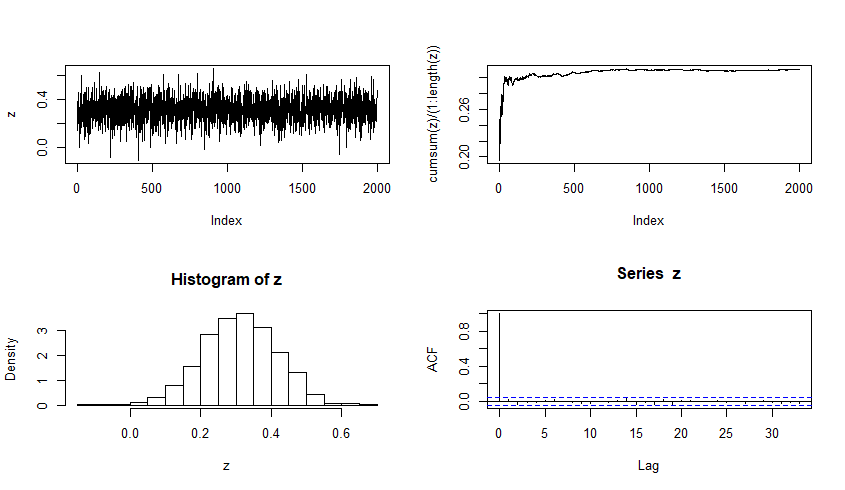
\includegraphics[width=0.9\linewidth]{Paper/images/271_genero_1mujer.png}
	\caption{ Cicloestación 271 - traceplot, promedios ergódicos, histograma de simulaciones y ACF para género femenino}
	\label{fig:pen_habs_penb271gen1}
\end{figure}
\newpage

En la gráfica anterior se observan las siguientes características:
\begin {itemize}
\item a) superior izquierda: la traza de la cadena para el caso del parámetro genero1. \item b)superior derecha: promedios ergódicos, donde se observa que la cadena convergió.
\item c) inferior izquierda: histograma de la función de densidad para el parámetro genero1.
\item d)inferior derecha: autocorrelación. Valores cercanos a cero indican que la simulaciones son casi independientes. 
\end {itemize}

Respecto al DIC se destacan los siguientes valores tras realizar el ajuste de los 15 modelos en cuestión:

\begin{table}[tbhp]
\centering
\caption{DIC obtenido en las simulaciones de Jags}
\label{tab:dic}
\begin{tabular}{@{}cccc@{}}
\toprule
Liga & Baja (estación 303) & Media (estación71) & Alta (estación 72) \\ \midrule
Canónica & 649.37 & 1,874.17 & 3,550.05 \\
Log-log & 616.07 & 1,860.16 & 3,572.36 \\
Clog-log & 590.22* & 1,830.15* &  3,502.97* \\
Logit & 664.00 & 1,857.25 & 3,556.08 \\
Probit & 591.48 & 1,891.04 & 4,043.04 \\ \bottomrule
\end{tabular}
\end{table}

Se destaca que en las tres estaciones, los modelos con mayor desempeño fueron aquellos que emplearon la liga $c-log-log$ 

\section{Interpretación de resultados}

De todo el análisis y modelos ajustados en las secciones previas; a continuación se presenta un resumen de las principales variables en donde se encontró significancia con respecto a la duración de los viajes con respecto al umbral especificado:

\begin{table}[tbhp]
\centering
\label{tab:param_resulta}
\begin{tabular}{@{}ccccc@{}}
\toprule
Parámetro & Valores & Estación 271 & Estación 72 & Estación 303 \\ \midrule
Género & 1 & + &  & + \\
Género & 2 & - &  & - \\
Hora & 9 &  &  & - \\
Día y hora & 2 y 10 &  &  & + \\
Día y hora & 1 y 11 & + &  &  \\ \bottomrule
\end{tabular}
\caption{Resumen de parámetros significativos en los modelos para las estaciones. Nota: los símbolos "+" y "-" denotan, respectivamente, que se obtuvo significancia positiva y negativa.}
\end{table}

Dentro del contexto de nuestro problema, de dicha tabla se desprende que:
\begin{itemize}
    \item En el caso de las cicloestaciones de demanda alta y baja consideradas, que un usuario pertenezca al género femenino es un factor positivo para que la duración de los viajes vaya más allá del umbral planteado por el programa. Esto es, las usuarias del Sistema Ecobici tienen una probabilidad positiva de realizar viajes que duren más de los 10 minutos; sin embargo esta tendencia no parece propia de la estación de demanda media.
    \item En contraste, para las cicloestaciones de demanda alta y baja consideradas, el que un usuario pertenezca al género masculino es un factor negativo para que duración de los viajes vaya más allá del umbral planteado por el programa propuesto. Ello significa que los usuarios (hombres) tienen una probabilidad baja de realizar viajes que duren más de los 10 minutos.
    \item En el caso de la cicloestación de baja demanda, un viaje que se inicie en el horario de las 9 de la mañana es un factor negativo para que duración de los viajes supere el umbral planteado con motivo del programa.
    \item Para la estación de baja demanda, el que un viaje inicie a las 10 am en el día martes es un factor positivo para que un viaje supere el umbral de tiempo especificado.
    \item Para la estación con demanda media considerada, el que un viaje se realice a las 11 de la mañana en los días lunes, es un factor positivo para que este dure más de 10 minutos.
    \end{itemize}

Del mismo modo, para ilustrar la significancia de los parámetros,se muestra el gráfico obtenido en JAGS mostrando el efecto significativo del género en la duración del viaje para la cicloestación 271.\footnote{Ver apéndice para observar los gráficos de significancia más representativos}

\begin{figure}[tbhp]
	\centering
	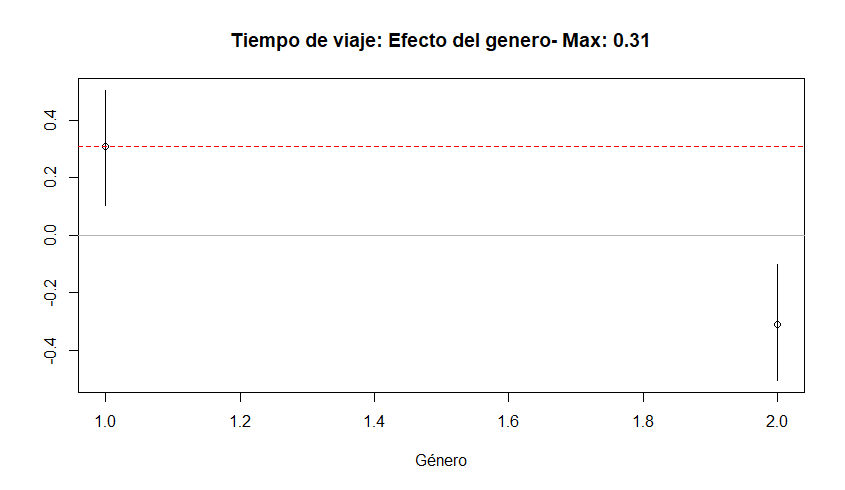
\includegraphics[width=0.9\linewidth]{Paper/images/271_efecto_genero.png}
	\caption{ Efecto del género en la duración del viaje para la cicloestación 271 }
	\label{fig:pen_habs_penb271gen1}
\end{figure}

Se observa que el genero femenino (1) tiene un efecto significativo en la duración de los viajes, indicando que los viajes de las mujeres para esta estación tienden a durar más. De forma contrario sucede para el género masculino(2).

\section{Consideraciones del problema a partir de resultados}

Del conjunto de factores significativos que se desprende del análisis exploratorio y de los modelos estadísticos bajo un enfoque bayesiano descrito en la secciones precedentes, parece importante tener en cuenta lo siguiente para el diseño del programa piloto que incentive el uso de la bicicleta como medio transporte a través del sistema Ecobici:
\begin{itemize}
  \item La mayoría de los usuarios del sistema Ecobici son hombres.
  \item En dos de las tres cicloestaciones estudiadas, hay un efecto positivo del género femenino sobre la duración del viaje, y un efecto negativo del género masculino, es decir, las mujeres tienden a hacer recorridos mayores a 10 minutos. Esto es, este género tiende a hacer viajes que duran mayor tiempo y podrían ser buenas candidatas  a emplear aún más esta clase de vehículos en su día a día.
  \item En una de las cicloestaciones (303) se observa que las 9 am tiene un efecto negativo sobre la duración del viaje, seguido por un efecto positivo a las 10 am, que se aprecia también a las 11 am en otra de las cicloestaciones (271). 
  
  Sería deseable extender esta última tendencia al resto de las estaciones del programa u otros horarios; es decir, que la bicicleta se use por más tiempo en los trayectos de la mañana (por ejemplo, en horarios previos a la entrada al trabajo) con una alternativa seria a recorrer distancias con otros medios, como el metro o metrobú.
  \end {itemize}


A partir de lo anterior, se estima pertinente implementar un programa piloto para incentivar el uso de la bicicleta, que contemple:
\begin{itemize}
  \item Descuento a mujeres en la inscripción al programa Ecobici, de manera que puedan usar en periodos más prolongados la bicicleta como un medio de viaje. Es decir, se plantea un incentivo de entrada para aumentar la cuota de mujeres, que, puede ser un factor a que se usen las bicicletas en periodos más prolongados,
  \item Ofrecer acumulación de puntos a usuarios que realicen viajes mayores a 10 minutos antes de las 9am, de manera que las personas opten por este medio en sus labores de mañana, en una tendencia mayor a la que se observa en ciertas estaciones.
  

Así, se pretende 1) disminuir el sesgo de género en el número de usuarios del sistema Ecobici, aprovechando el efecto positivo observado del género femenino; además, 2) se busca fomentar que más usuarios sustituyan una parte de su trayecto diario por un trayecto en bicicleta, en lugar de utilizar otros medios de transporte, permitiéndoles así mejorar su salud y condición física, y ayudar a reducir los congestionamientos, disminuyendo con ello el estrés y la sobrecarga de otros medios de transporte público. 
\end{itemize}

\section{Conclusiones}

\begin{itemize}
    \item En este documento se ha realizado un análisis ajustando modelos a un conjunto de datos de los viajes que los usuarios del Sistema Ecobicis realizaron en Octubre de 2019.
    \item  A partir de dicha información se realizó un análisis estadístico inferencial de dicha base de datos con base en la teoría bayesiana, en el cual se ajustaron un conjunto de modelos para tres estaciones elegidas con base en el perfil de demanda de viajes iniciados en estas. En concreto, se trabajó con 1) un conjunto de modelos de tipo Bernoulli donde la variable explicativa es de tipo categórica, que refiere a si los viajes de los usuarios fueron superiores a un umbral de tiempo, considerando las mismas covariables de los modelos anteriores y las covariables son el resto de características de los usuarios y del viajes (es decir, las cicloestaciones de origen y destino, la fecha y hora de los mismos).
    \item Para el ajuste del modelo de tipo Bernoulli se exploraron variantes del mismo empleando diferentes funciones liga, a saber, 1) logit, 2) probit, 3) log-log y 4) log-log complementario; encontrándose que ésta última es la que mejor se ajusta al modelo al considerar el DIC.
    \item Finalmente, se encontraron diversos factores significativos en la duración de los viajes más allá de un umbral especificado, del cual se desprendieron medidas que pueden adoptarse en un programa piloto para incentivar el uso de la bicicleta a través de Sistemas de Ecobicis, tanto en número de viajes como en duración de los mismos.
\end{itemize}

\bibliography{ilcss-sample}

\begin{appendices}


	\section{Figuras}


\begin{figure}[tbhp]
	\centering
	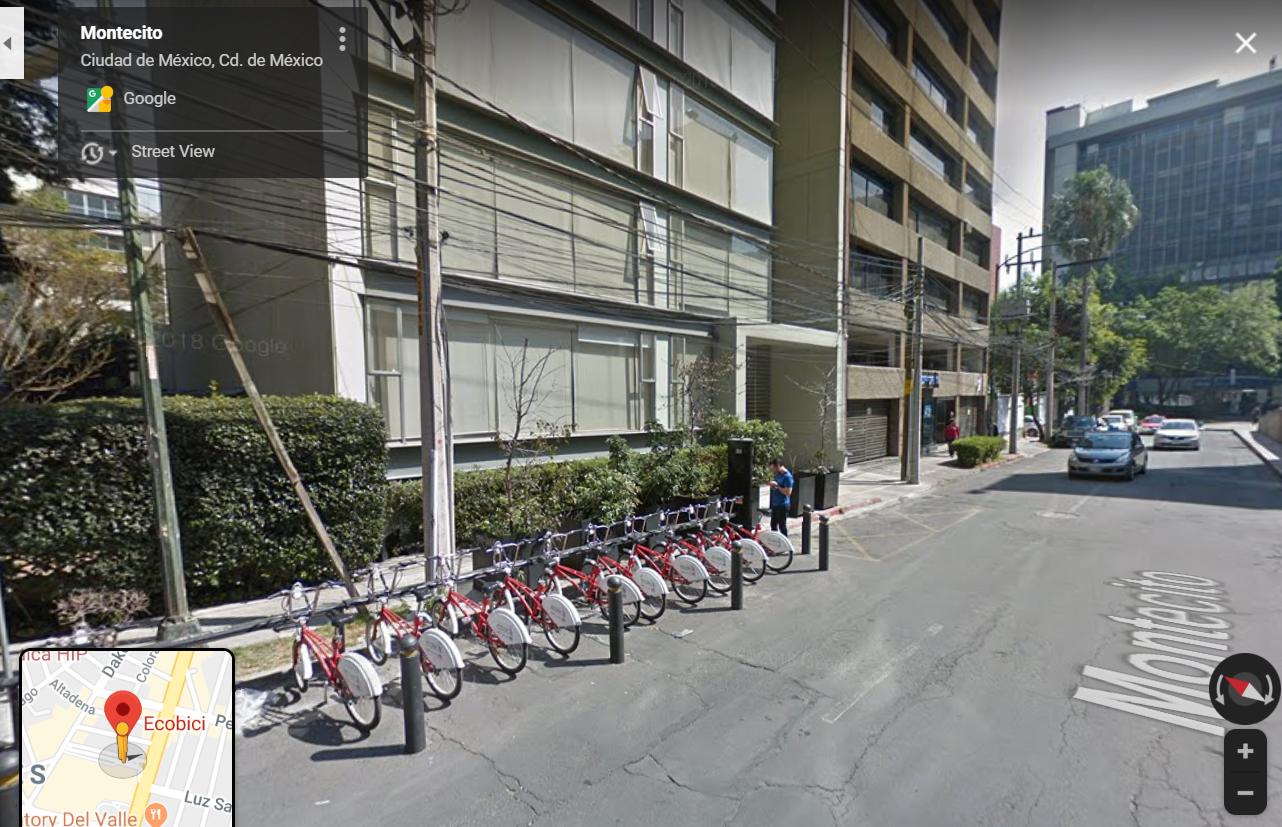
\includegraphics[width=0.9\linewidth]{Paper/images/estacion303.png}
	\caption{Cicloestación 303, Montesito-Avenida Insurgentes}
	\label{fig:pen_habs_penbc303}
\end{figure}
\begin{figure}[tbhp]
	\centering
	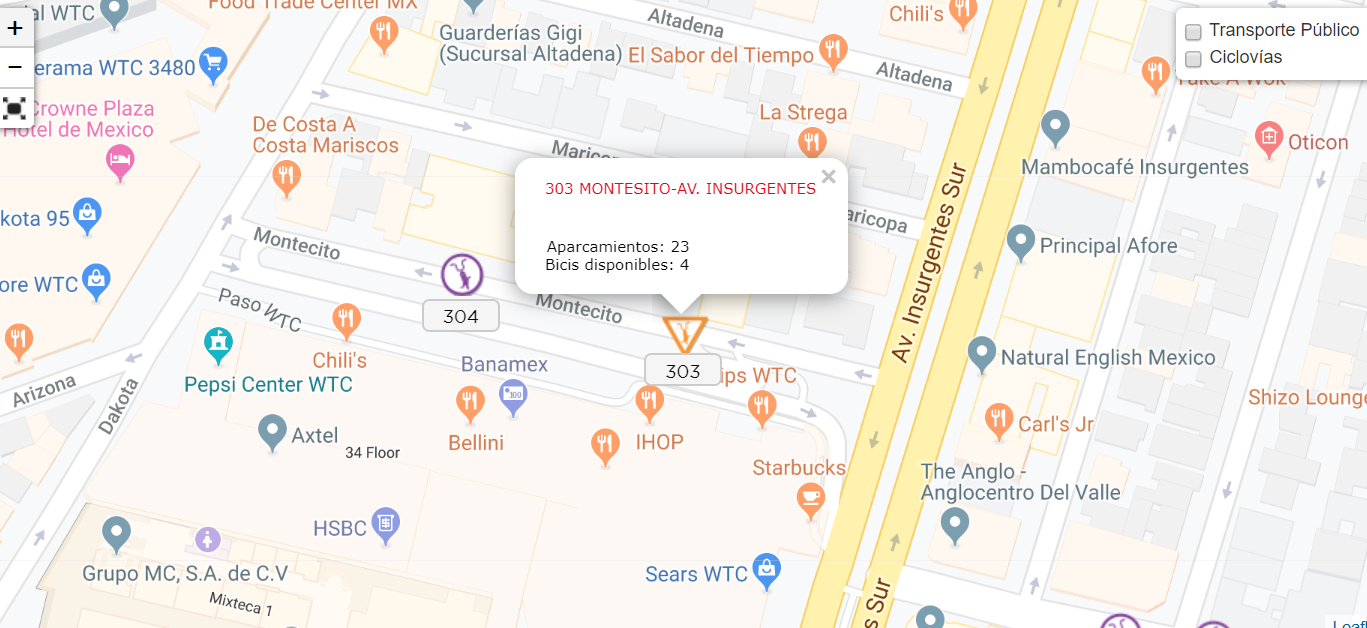
\includegraphics[width=0.9\linewidth]{Paper/images/estacion303_mapa.png}
	\caption{ Localización de la cicloestación 303, Montesito-Avenida Insurgentes}
	\label{fig:pen_habs_penbc303loc}
\end{figure}


\begin{figure}[tbhp]
	\centering
	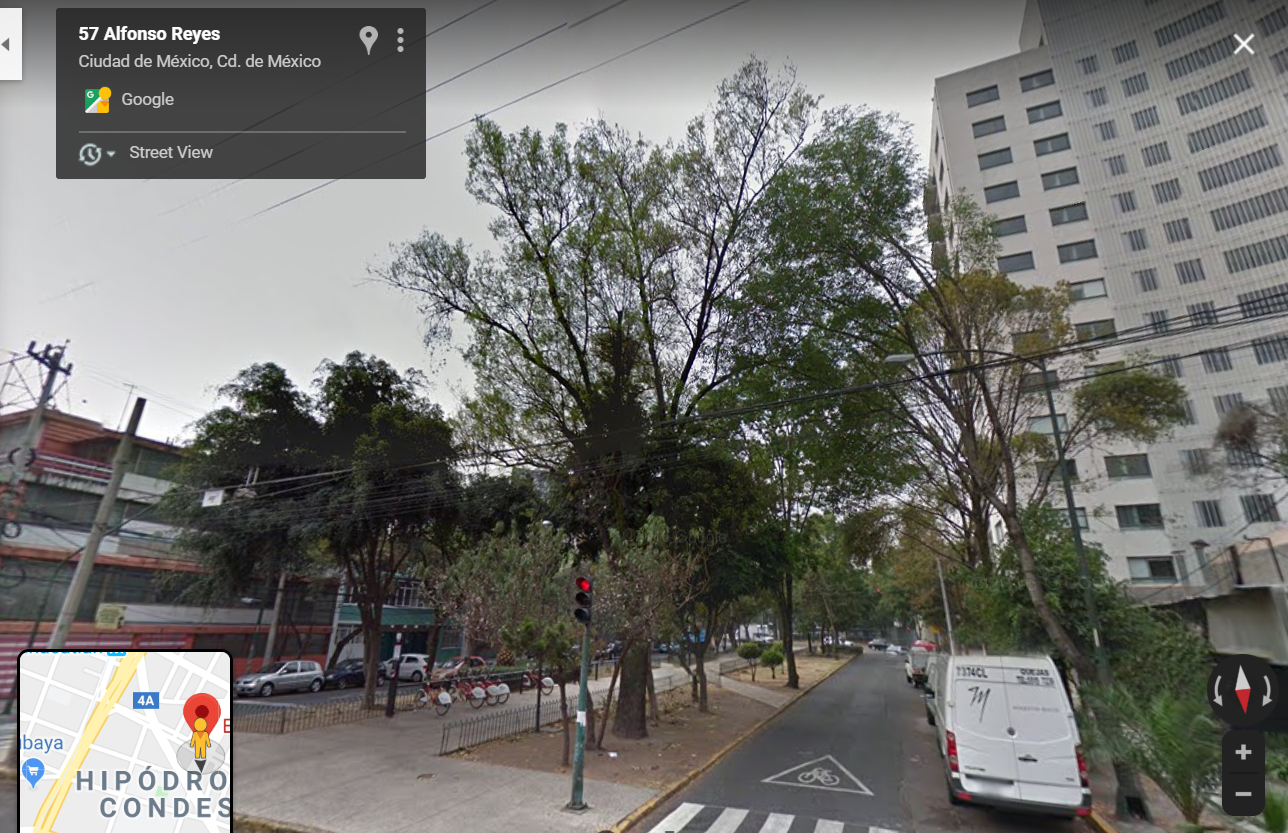
\includegraphics[width=0.9\linewidth]{Paper/images/estacion72.png}
	\caption{Cicloestación 72,Mazatlán-Alfonso Reyes}
	\label{fig:pen_habs_penbc72}
\end{figure}
\begin{figure}[tbhp]
	\centering
	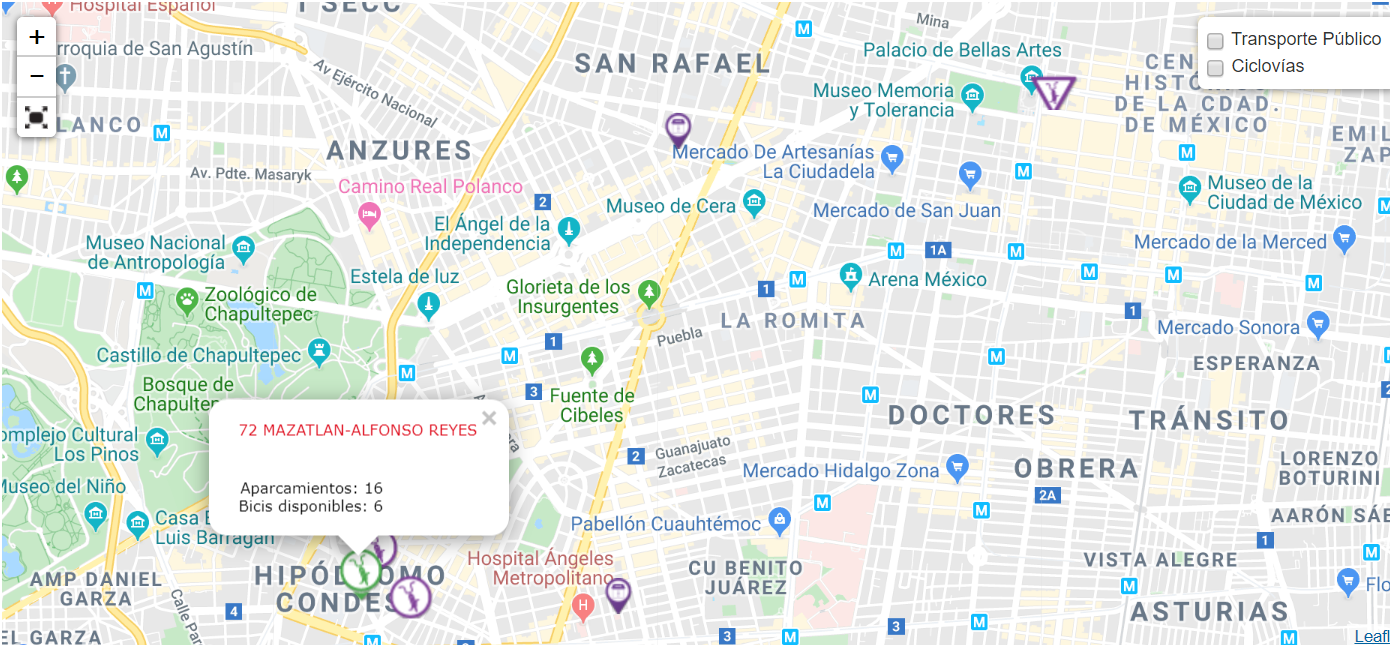
\includegraphics[width=0.9\linewidth]{Paper/images/estacion72_mapa.png}
	\caption{ Localización de la cicloestación 72, Mazatlán-Alfonso Reyes}
	\label{fig:pen_habs_penbc72loc}
\end{figure}

\begin{figure}[tbhp]
	\centering
	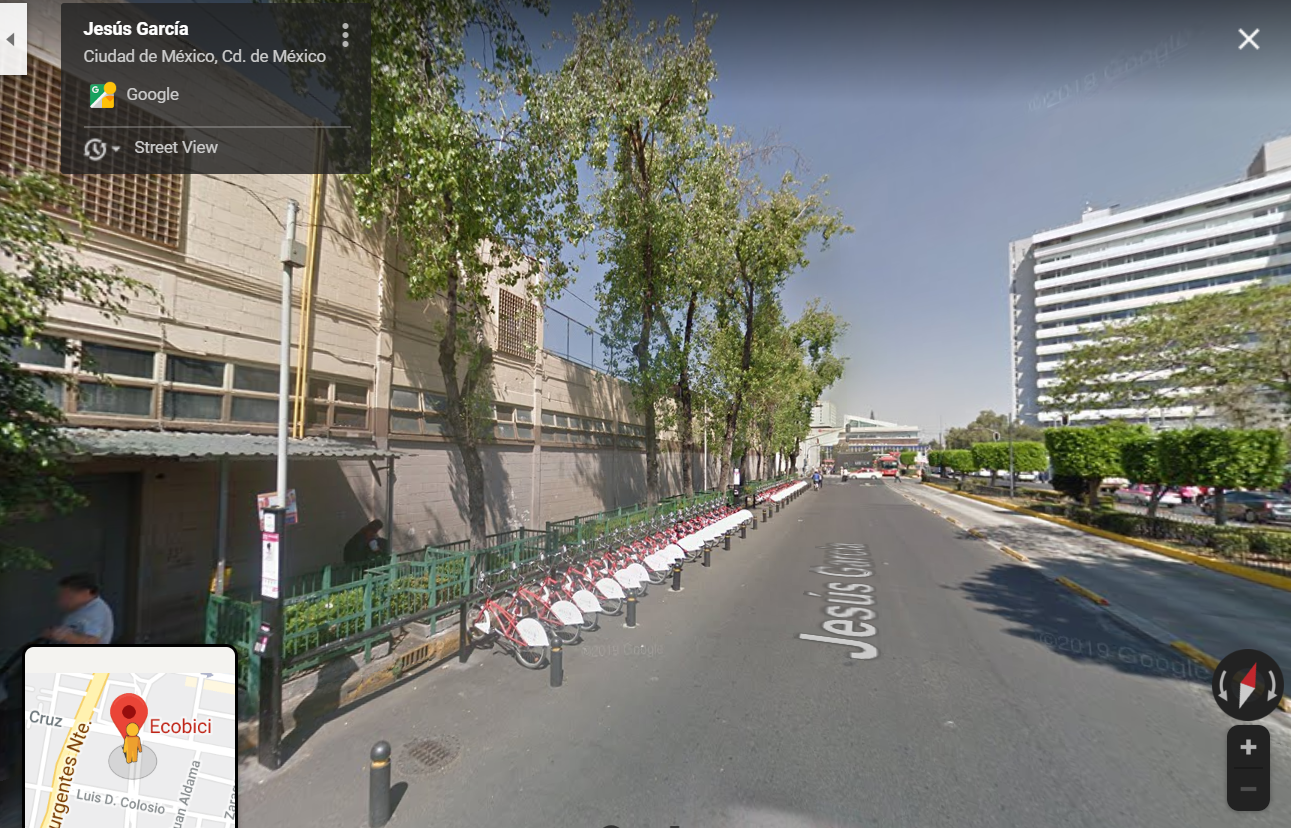
\includegraphics[width=0.9\linewidth]{Paper/images/estacion271.png}
	\caption{Cicloestación 271, Avenida Central-J.Meneses}
	\label{fig:pen_habs_penbc271}
\end{figure}
\begin{figure}[tbhp]
	\centering
	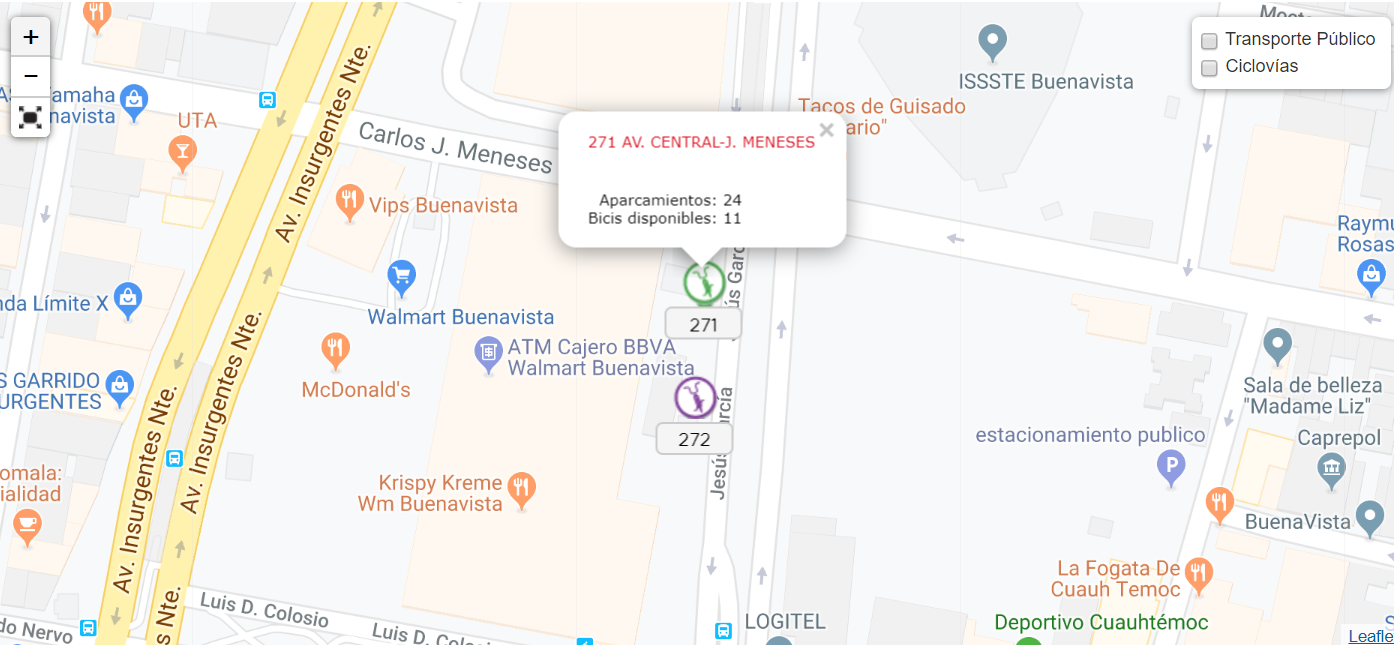
\includegraphics[width=0.9\linewidth]{Paper/images/estacion271_mapa.png}
	\caption{ Localización de la cicloestación 271, Avenida Central-J.Meneses}
	\label{fig:pen_habs_penbc271loc}
\end{figure}
\begin{figure}[tbhp]
	\centering
	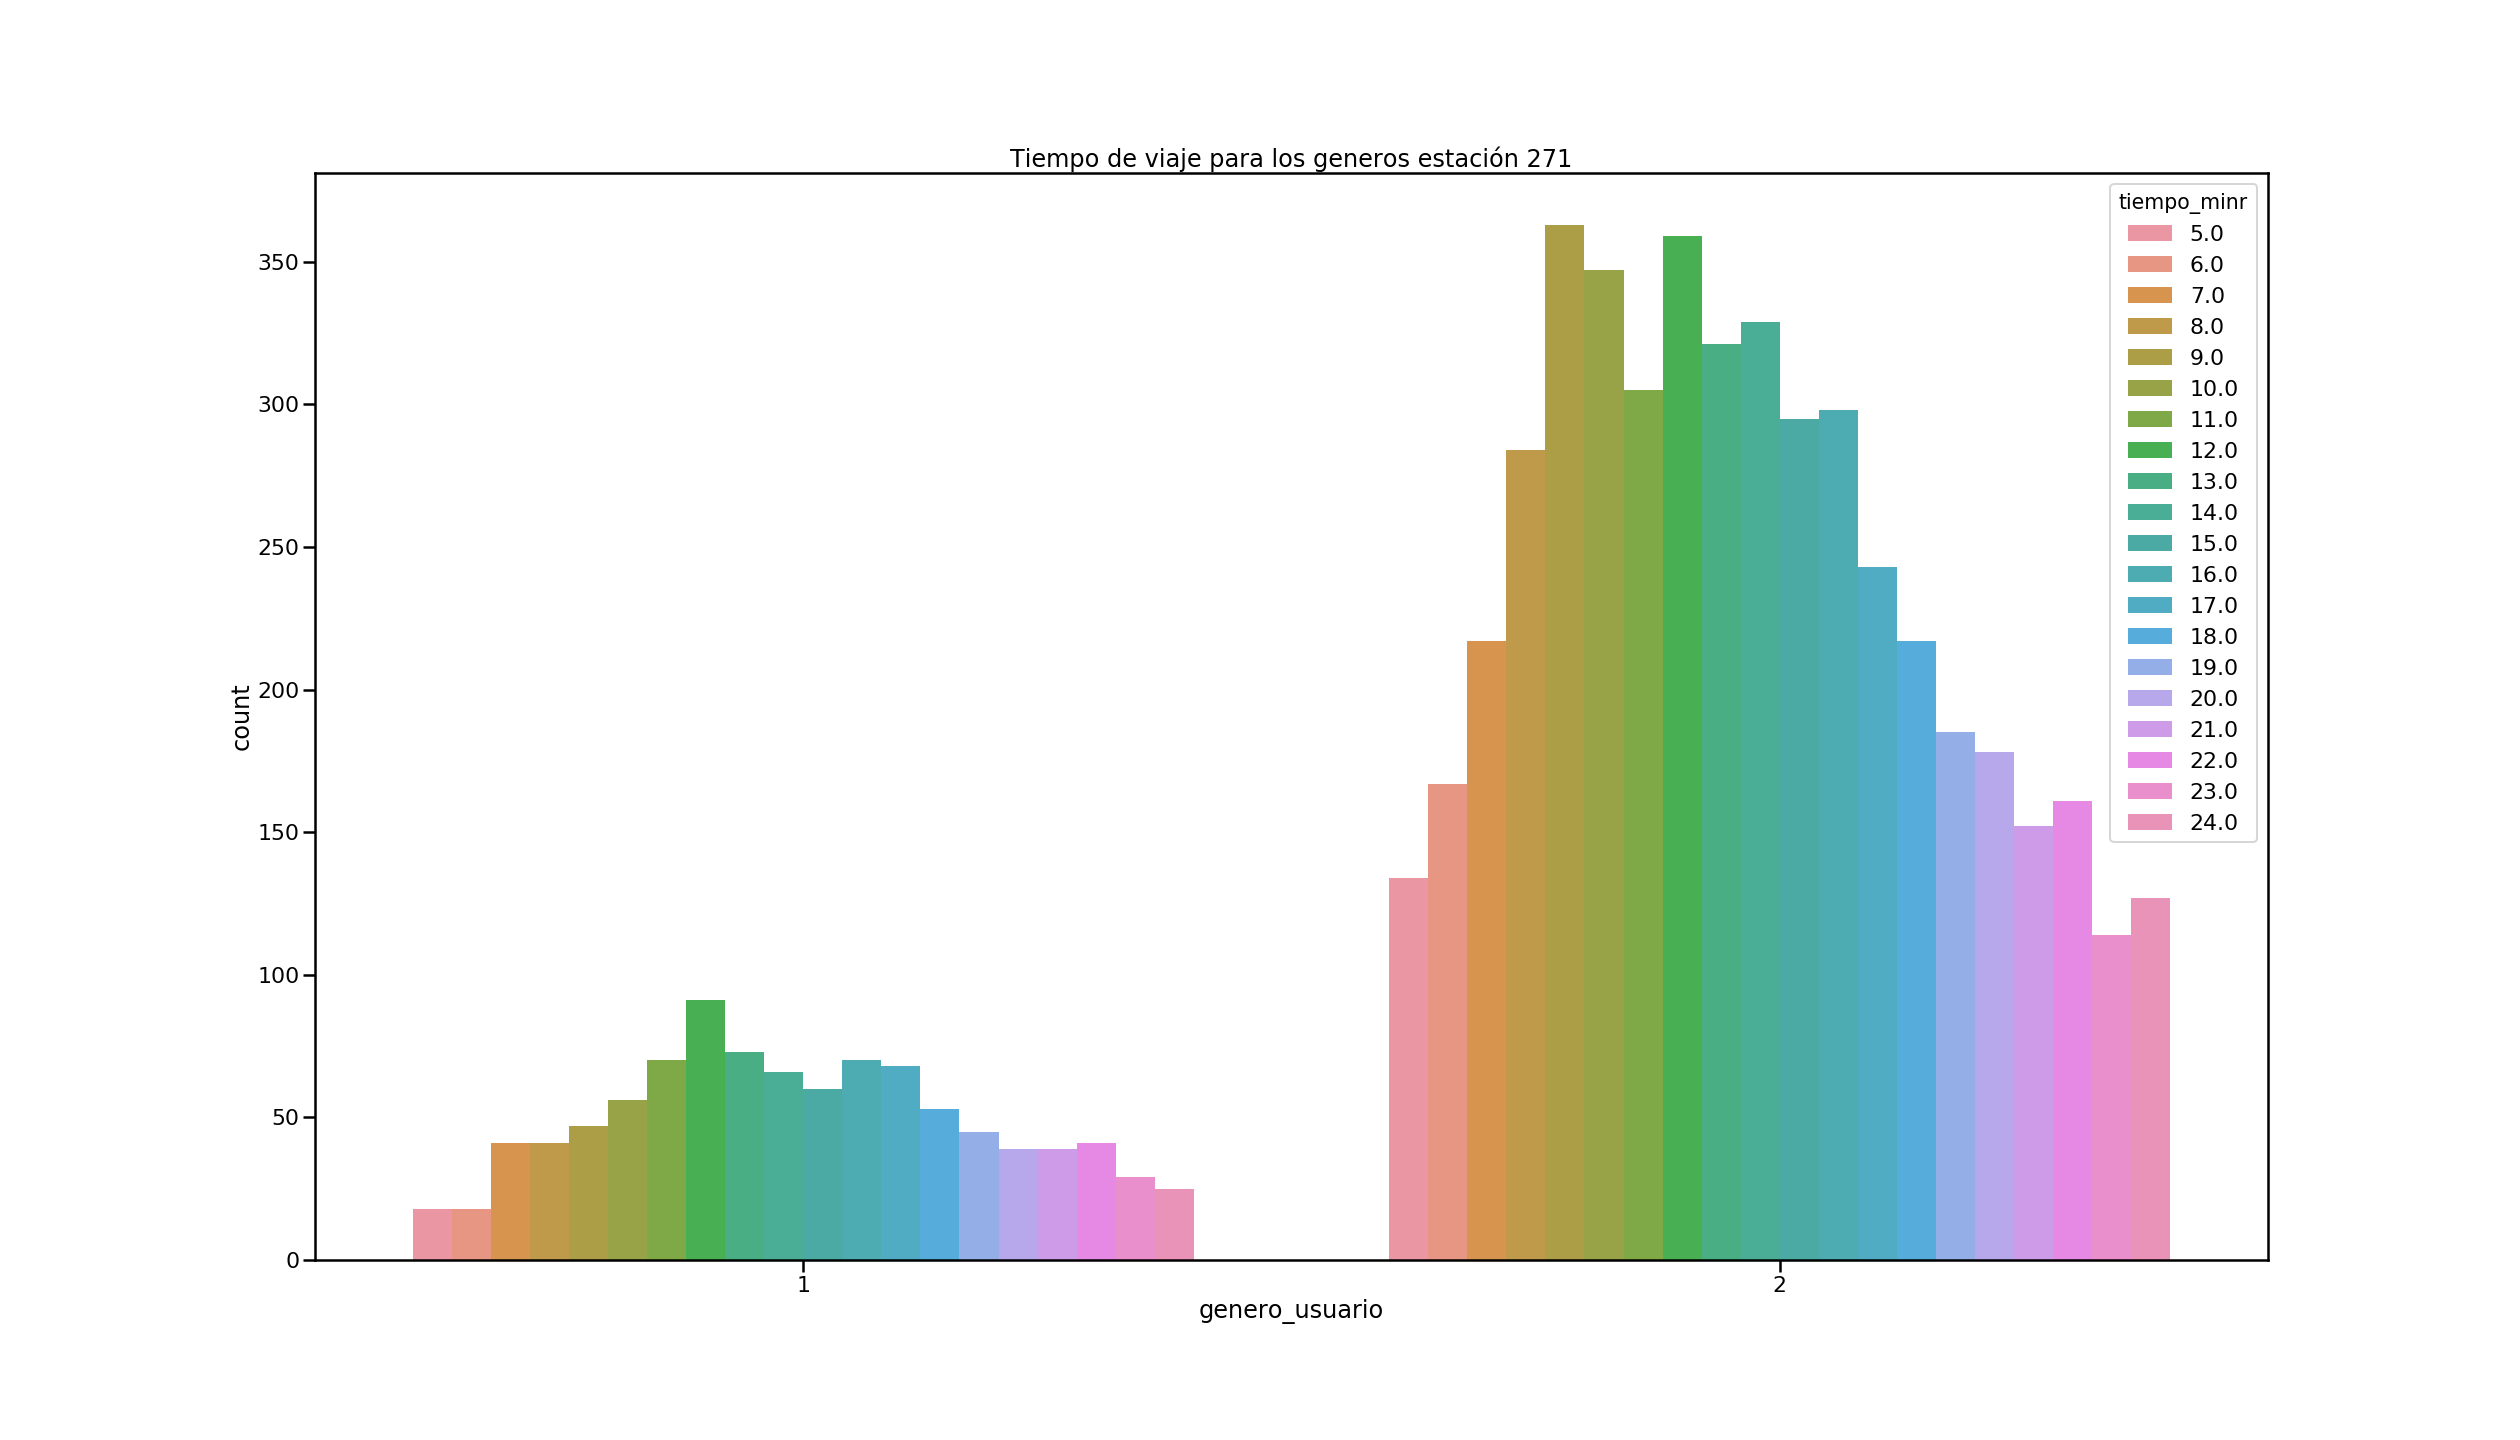
\includegraphics[width=0.9\linewidth]{Paper/images/tiempo_genero271.png}
	\caption{ Tiempos de viaje para ambos géneros en la estación 271}
	\label{fig:pen_habs_penbcGenero}
\end{figure}
\begin{figure}[tbhp]
	\centering
	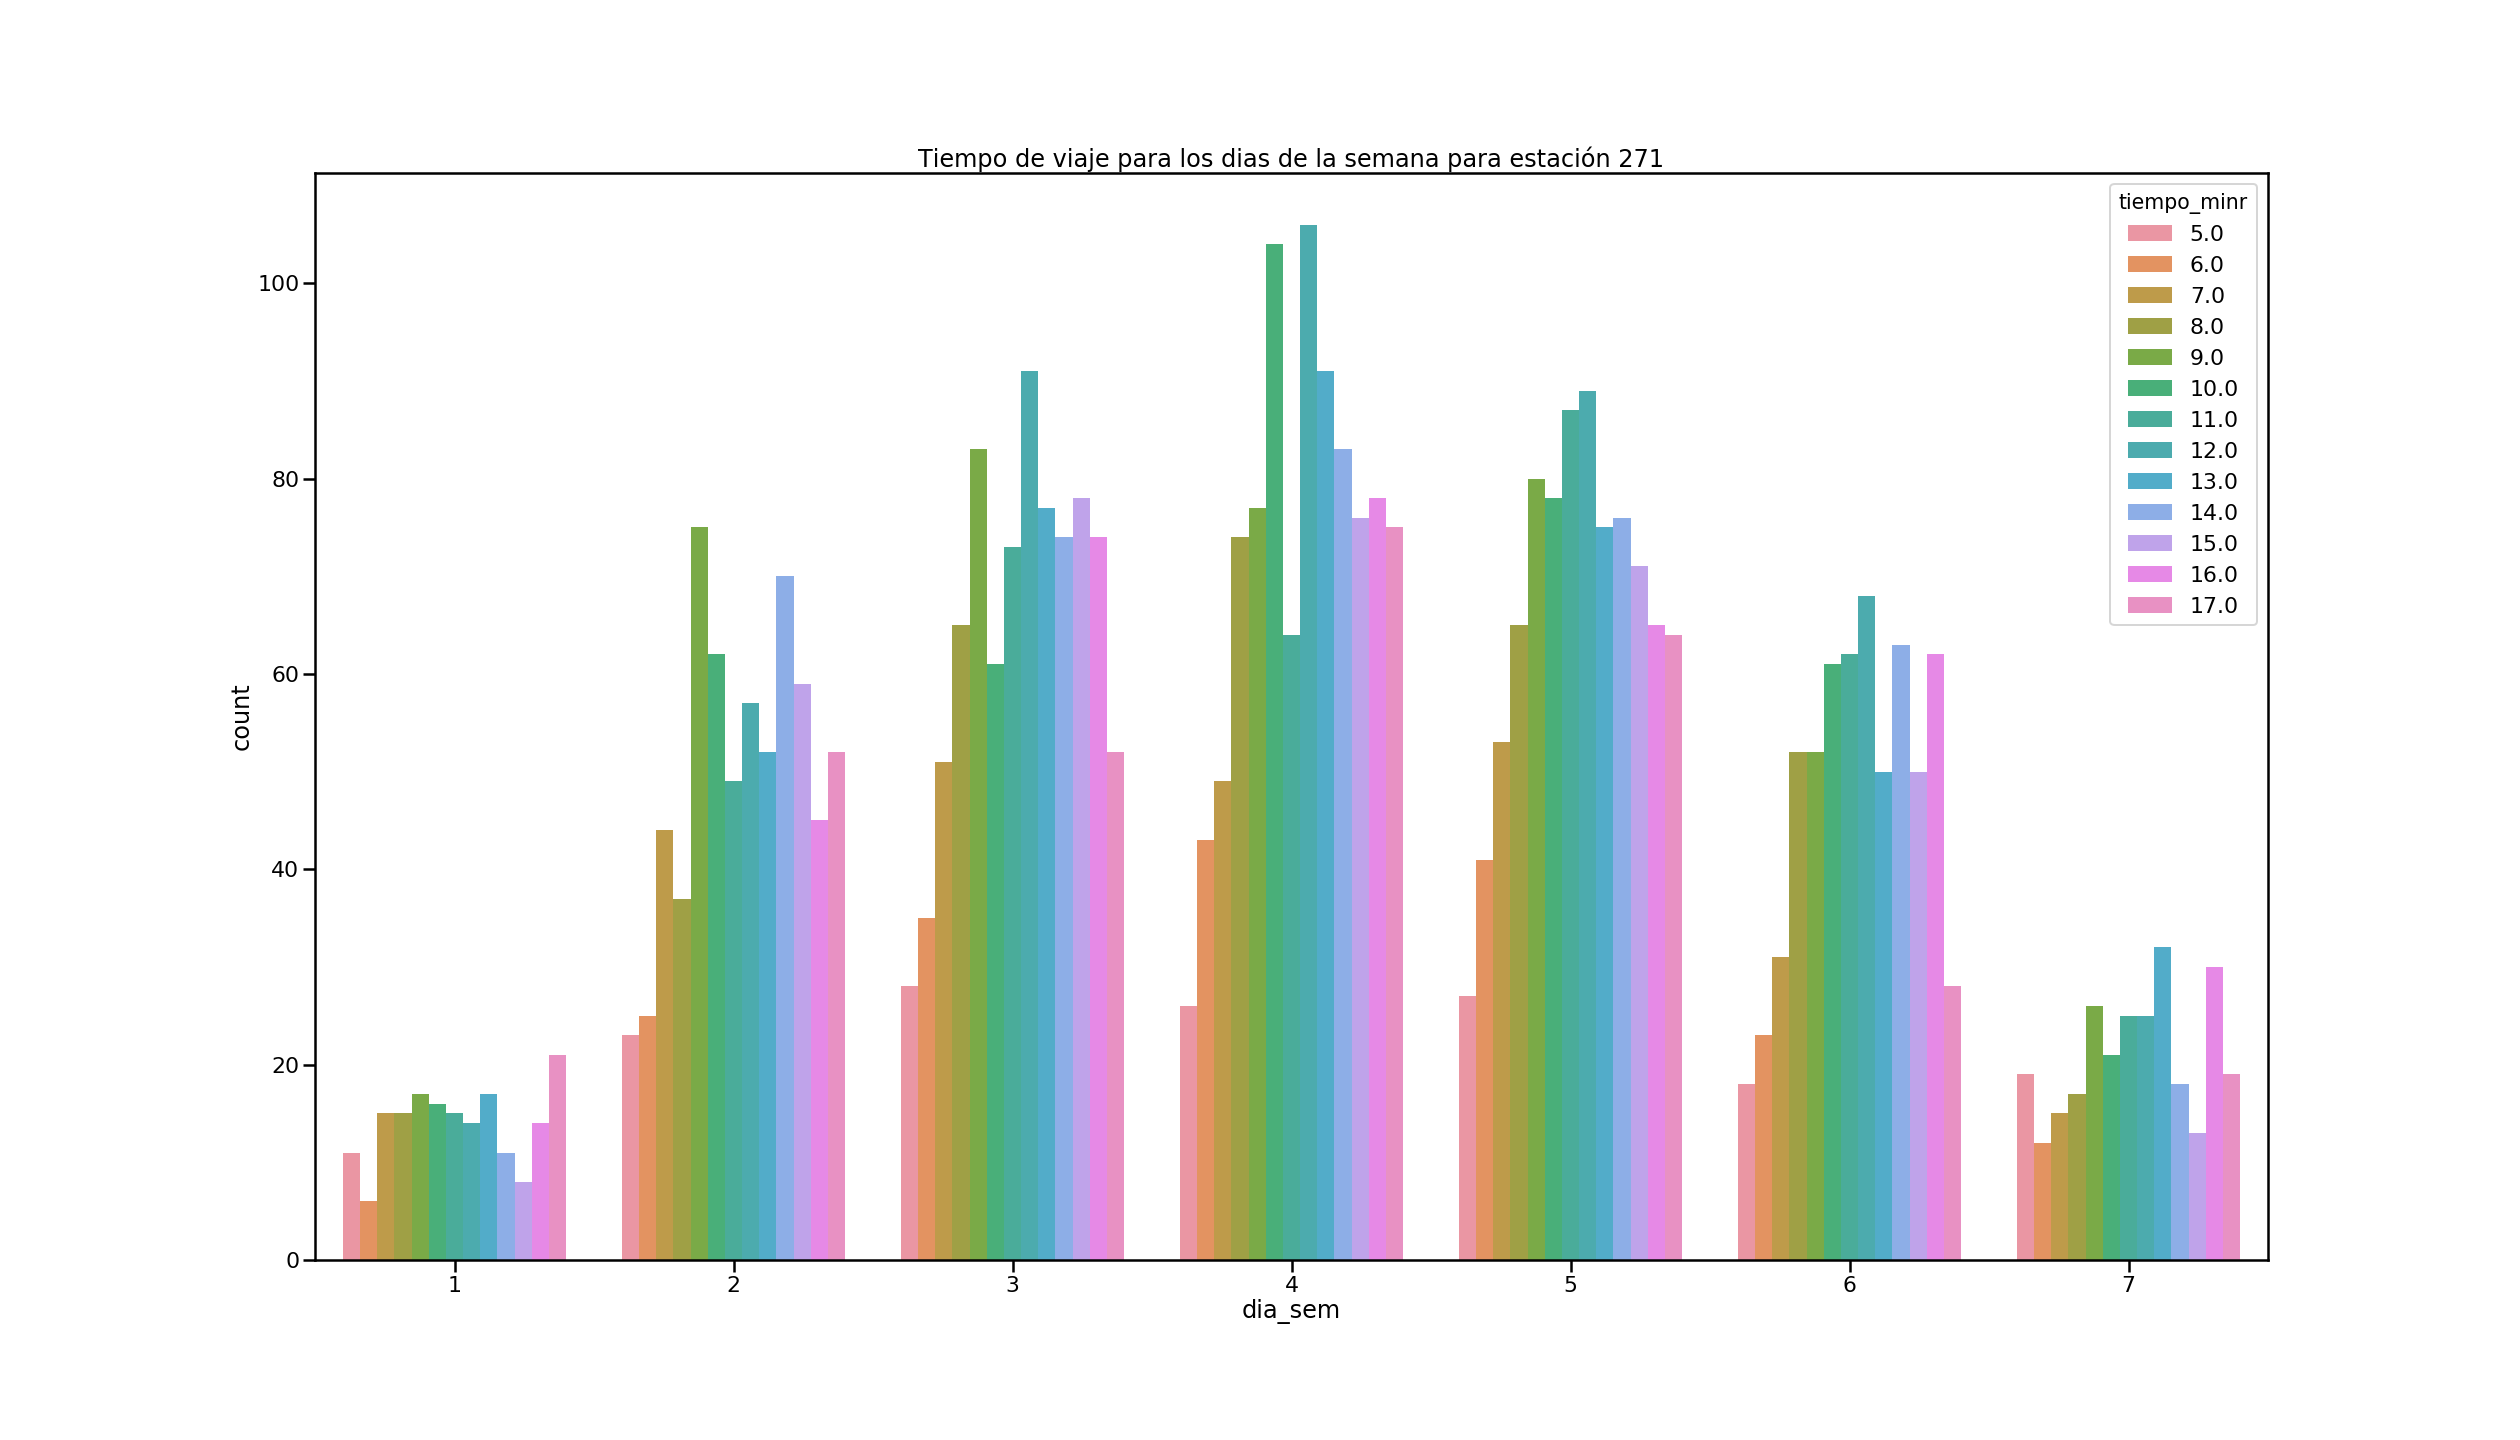
\includegraphics[width=0.9\linewidth]{Paper/images/tiempo_dias_semana_271.png}
	\caption{ Tiempos de viaje días de la semana en la estación 271}
	\label{fig:pen_habs_penbcDias}
\end{figure}
\begin{figure}[tbhp]
	\centering
	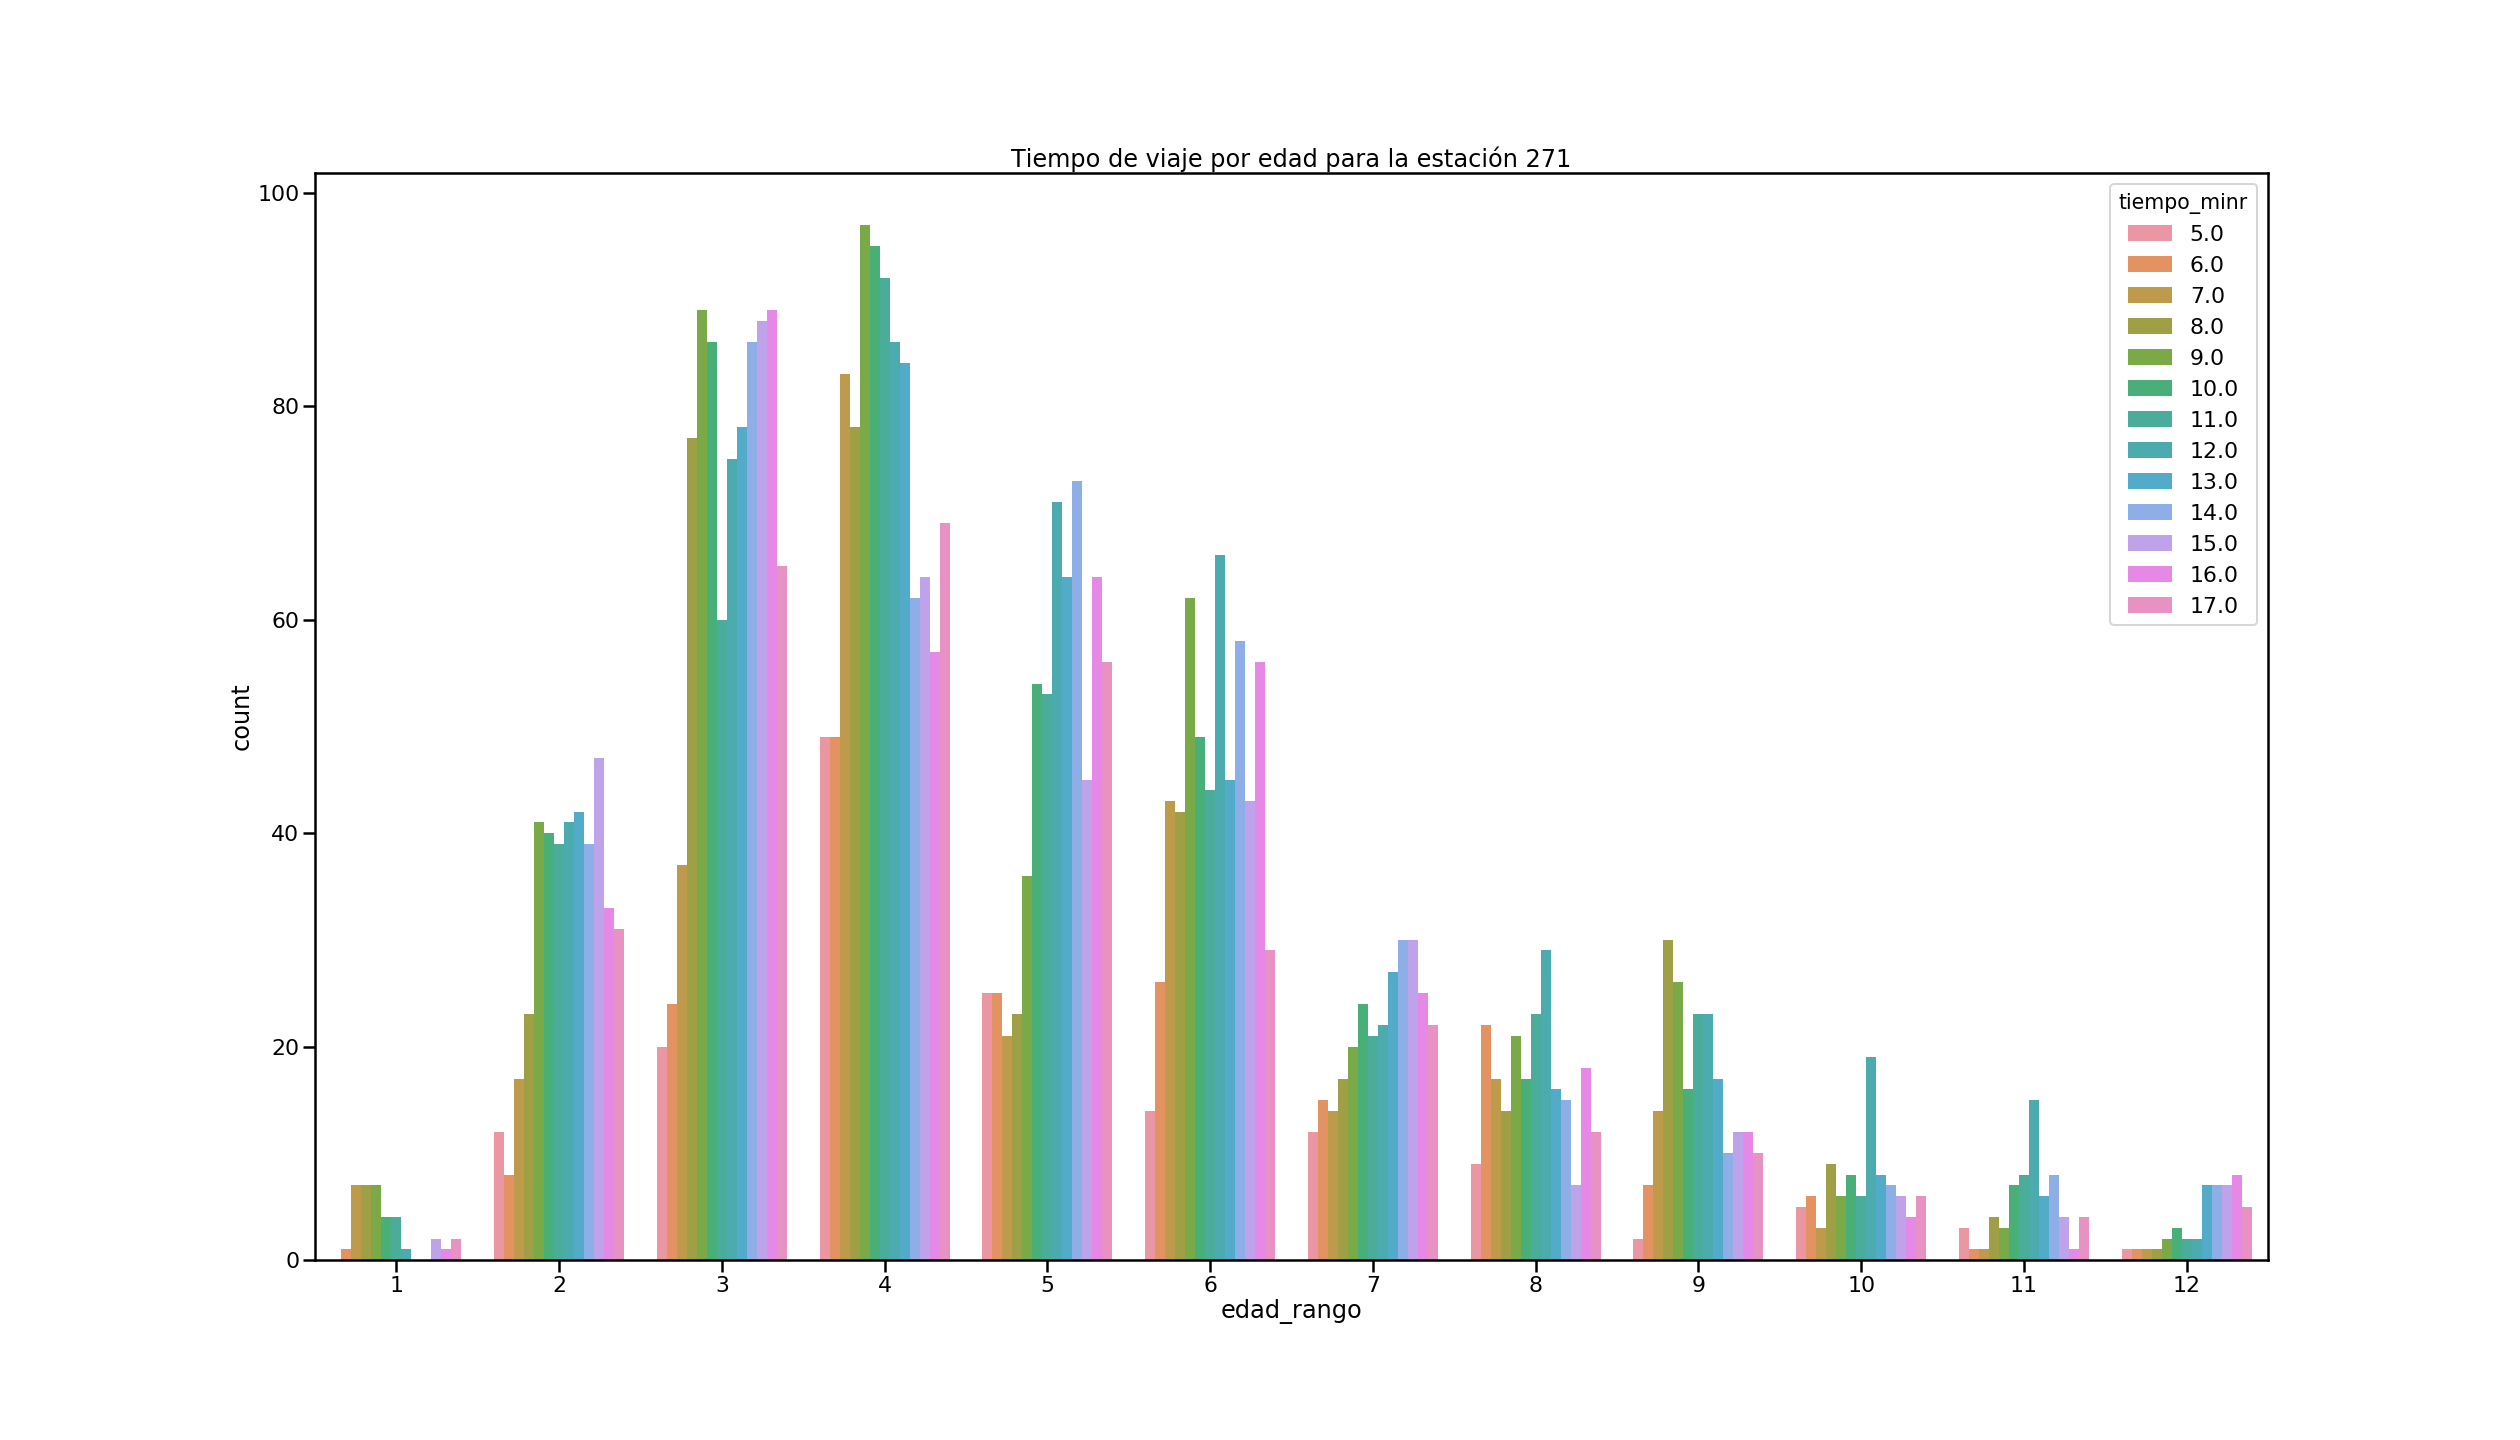
\includegraphics[width=0.9\linewidth]{Paper/images/tiempo_edad_271.png}
	\caption{ Tiempos de viaje por edad en la estación 271}
	\label{fig:pen_habs_penbcEdad}
\end{figure}
\begin{figure}[tbhp]
	\centering
	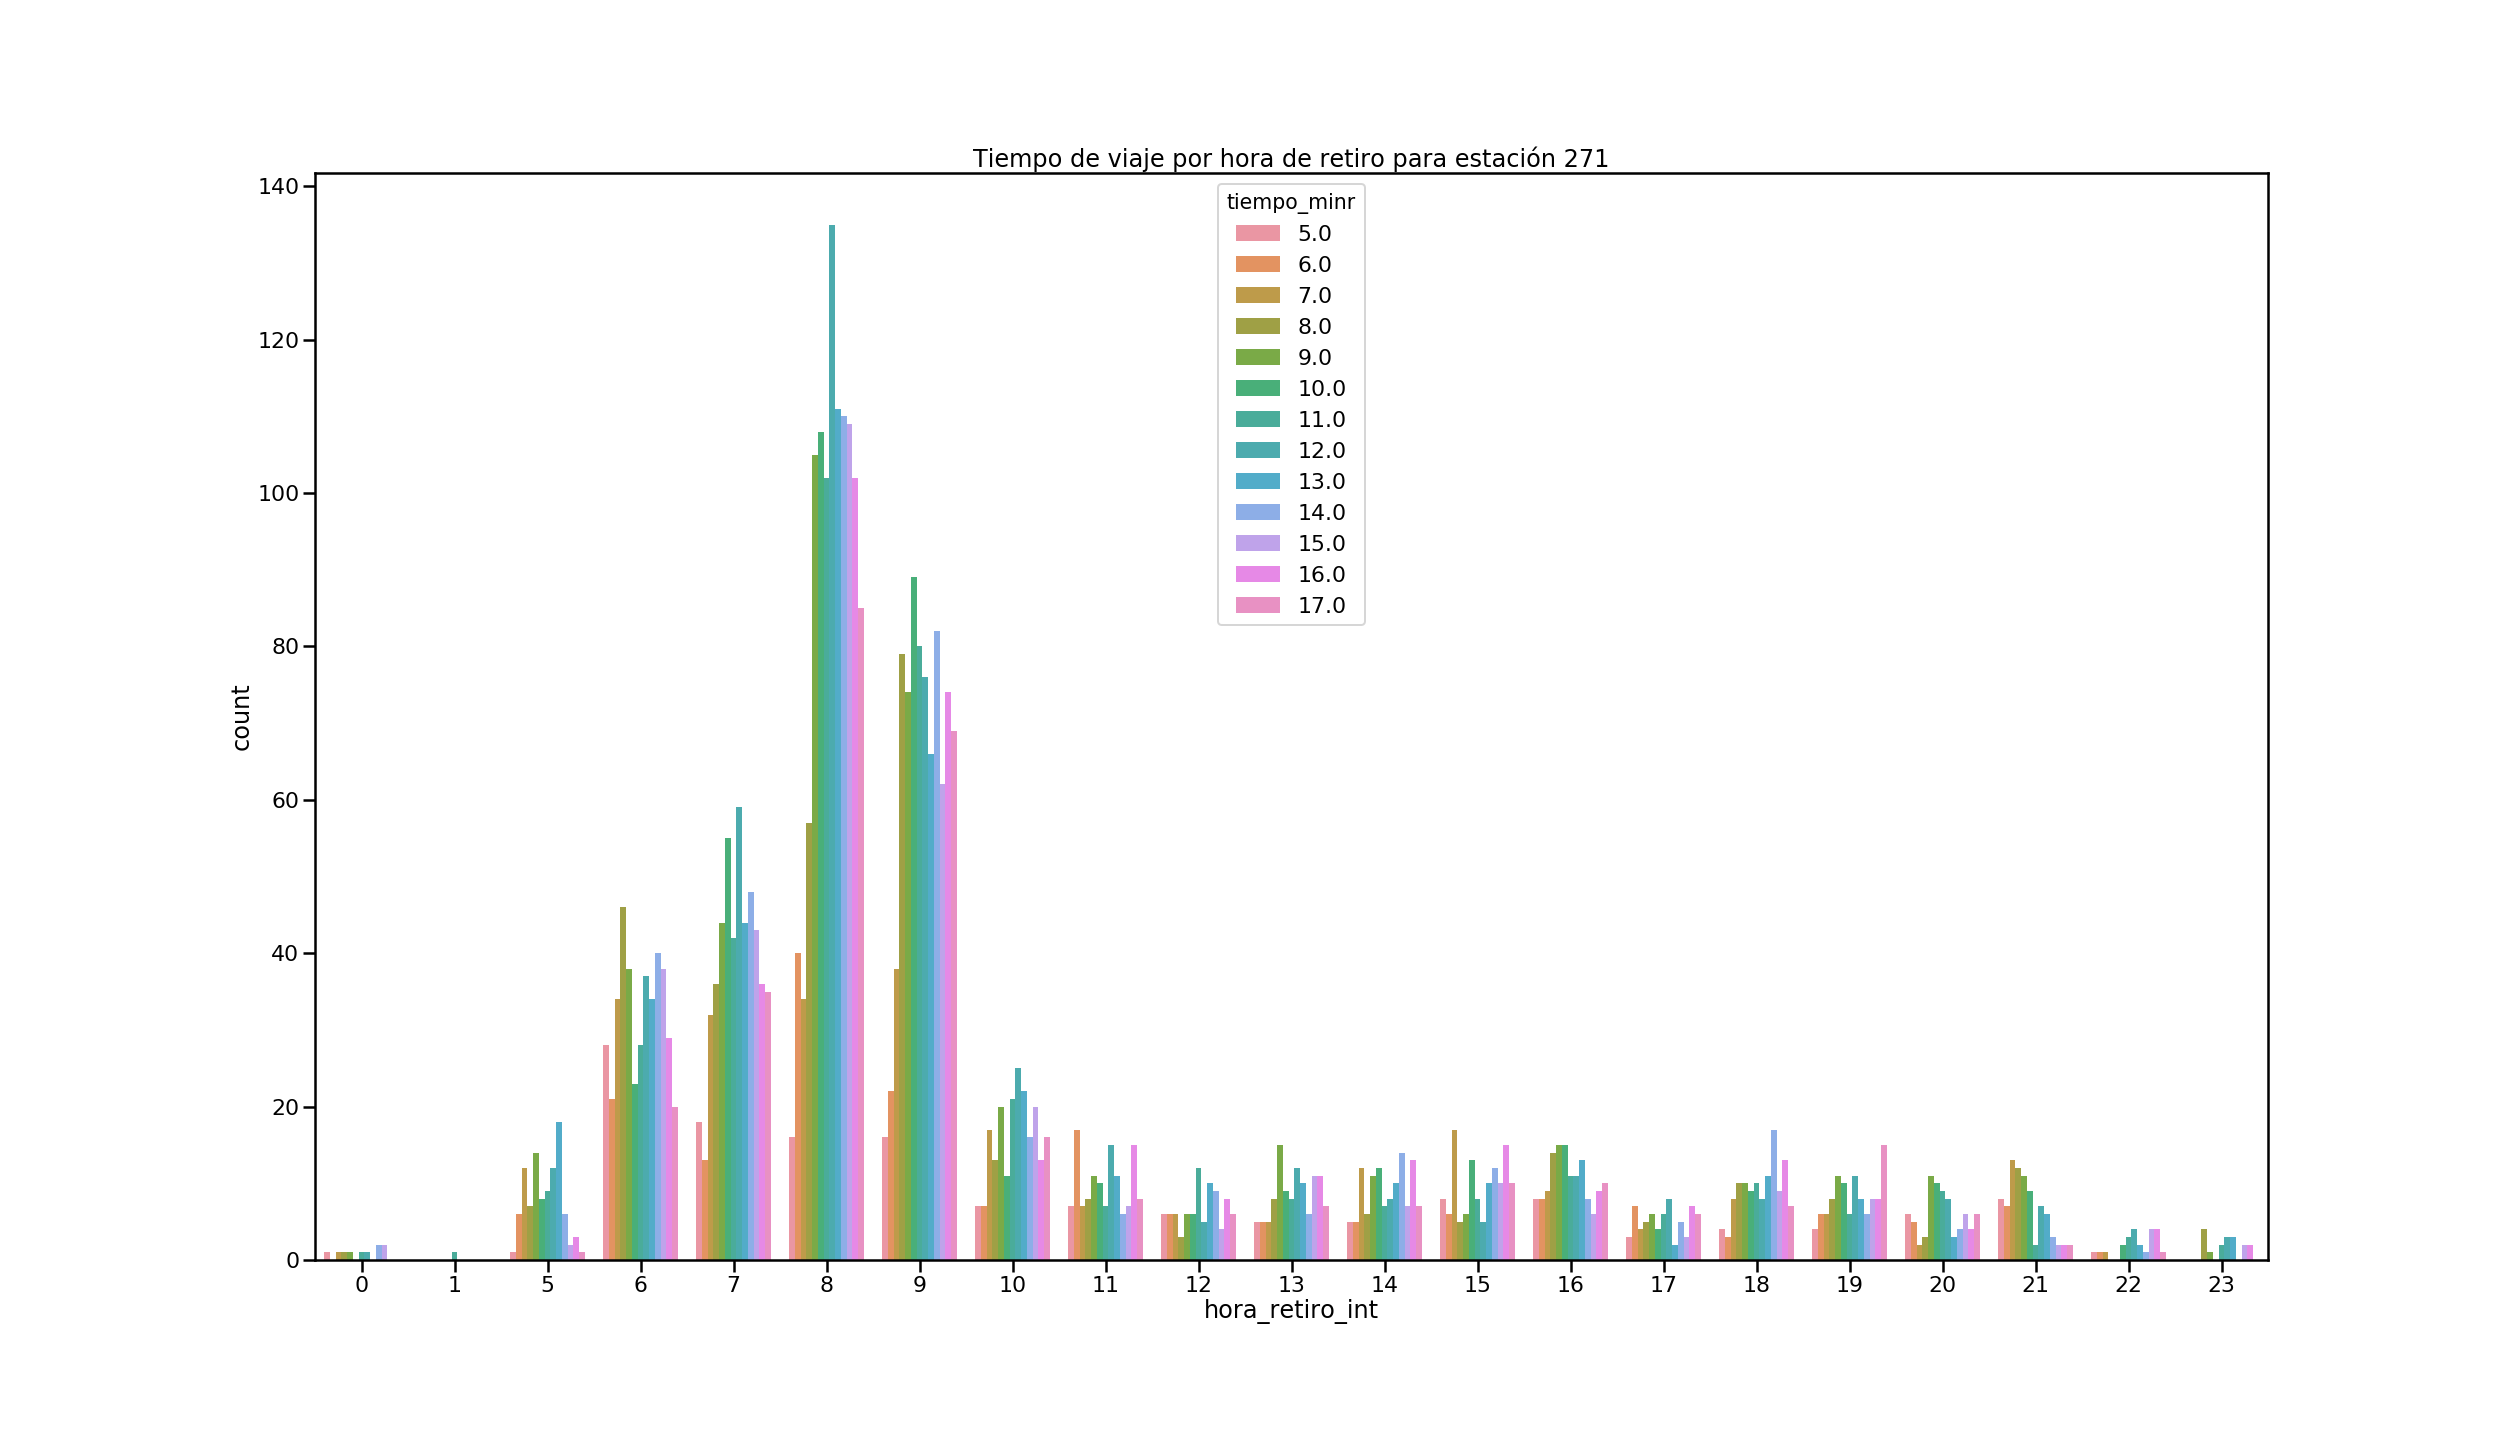
\includegraphics[width=0.9\linewidth]{Paper/images/tiempo_horas_271.png}
	\caption{ Tiempos de viaje por edad en la estación 271}
	\label{fig:pen_habs_penbcHoras}
\end{figure}
\begin{figure}[tbhp]
	\centering
	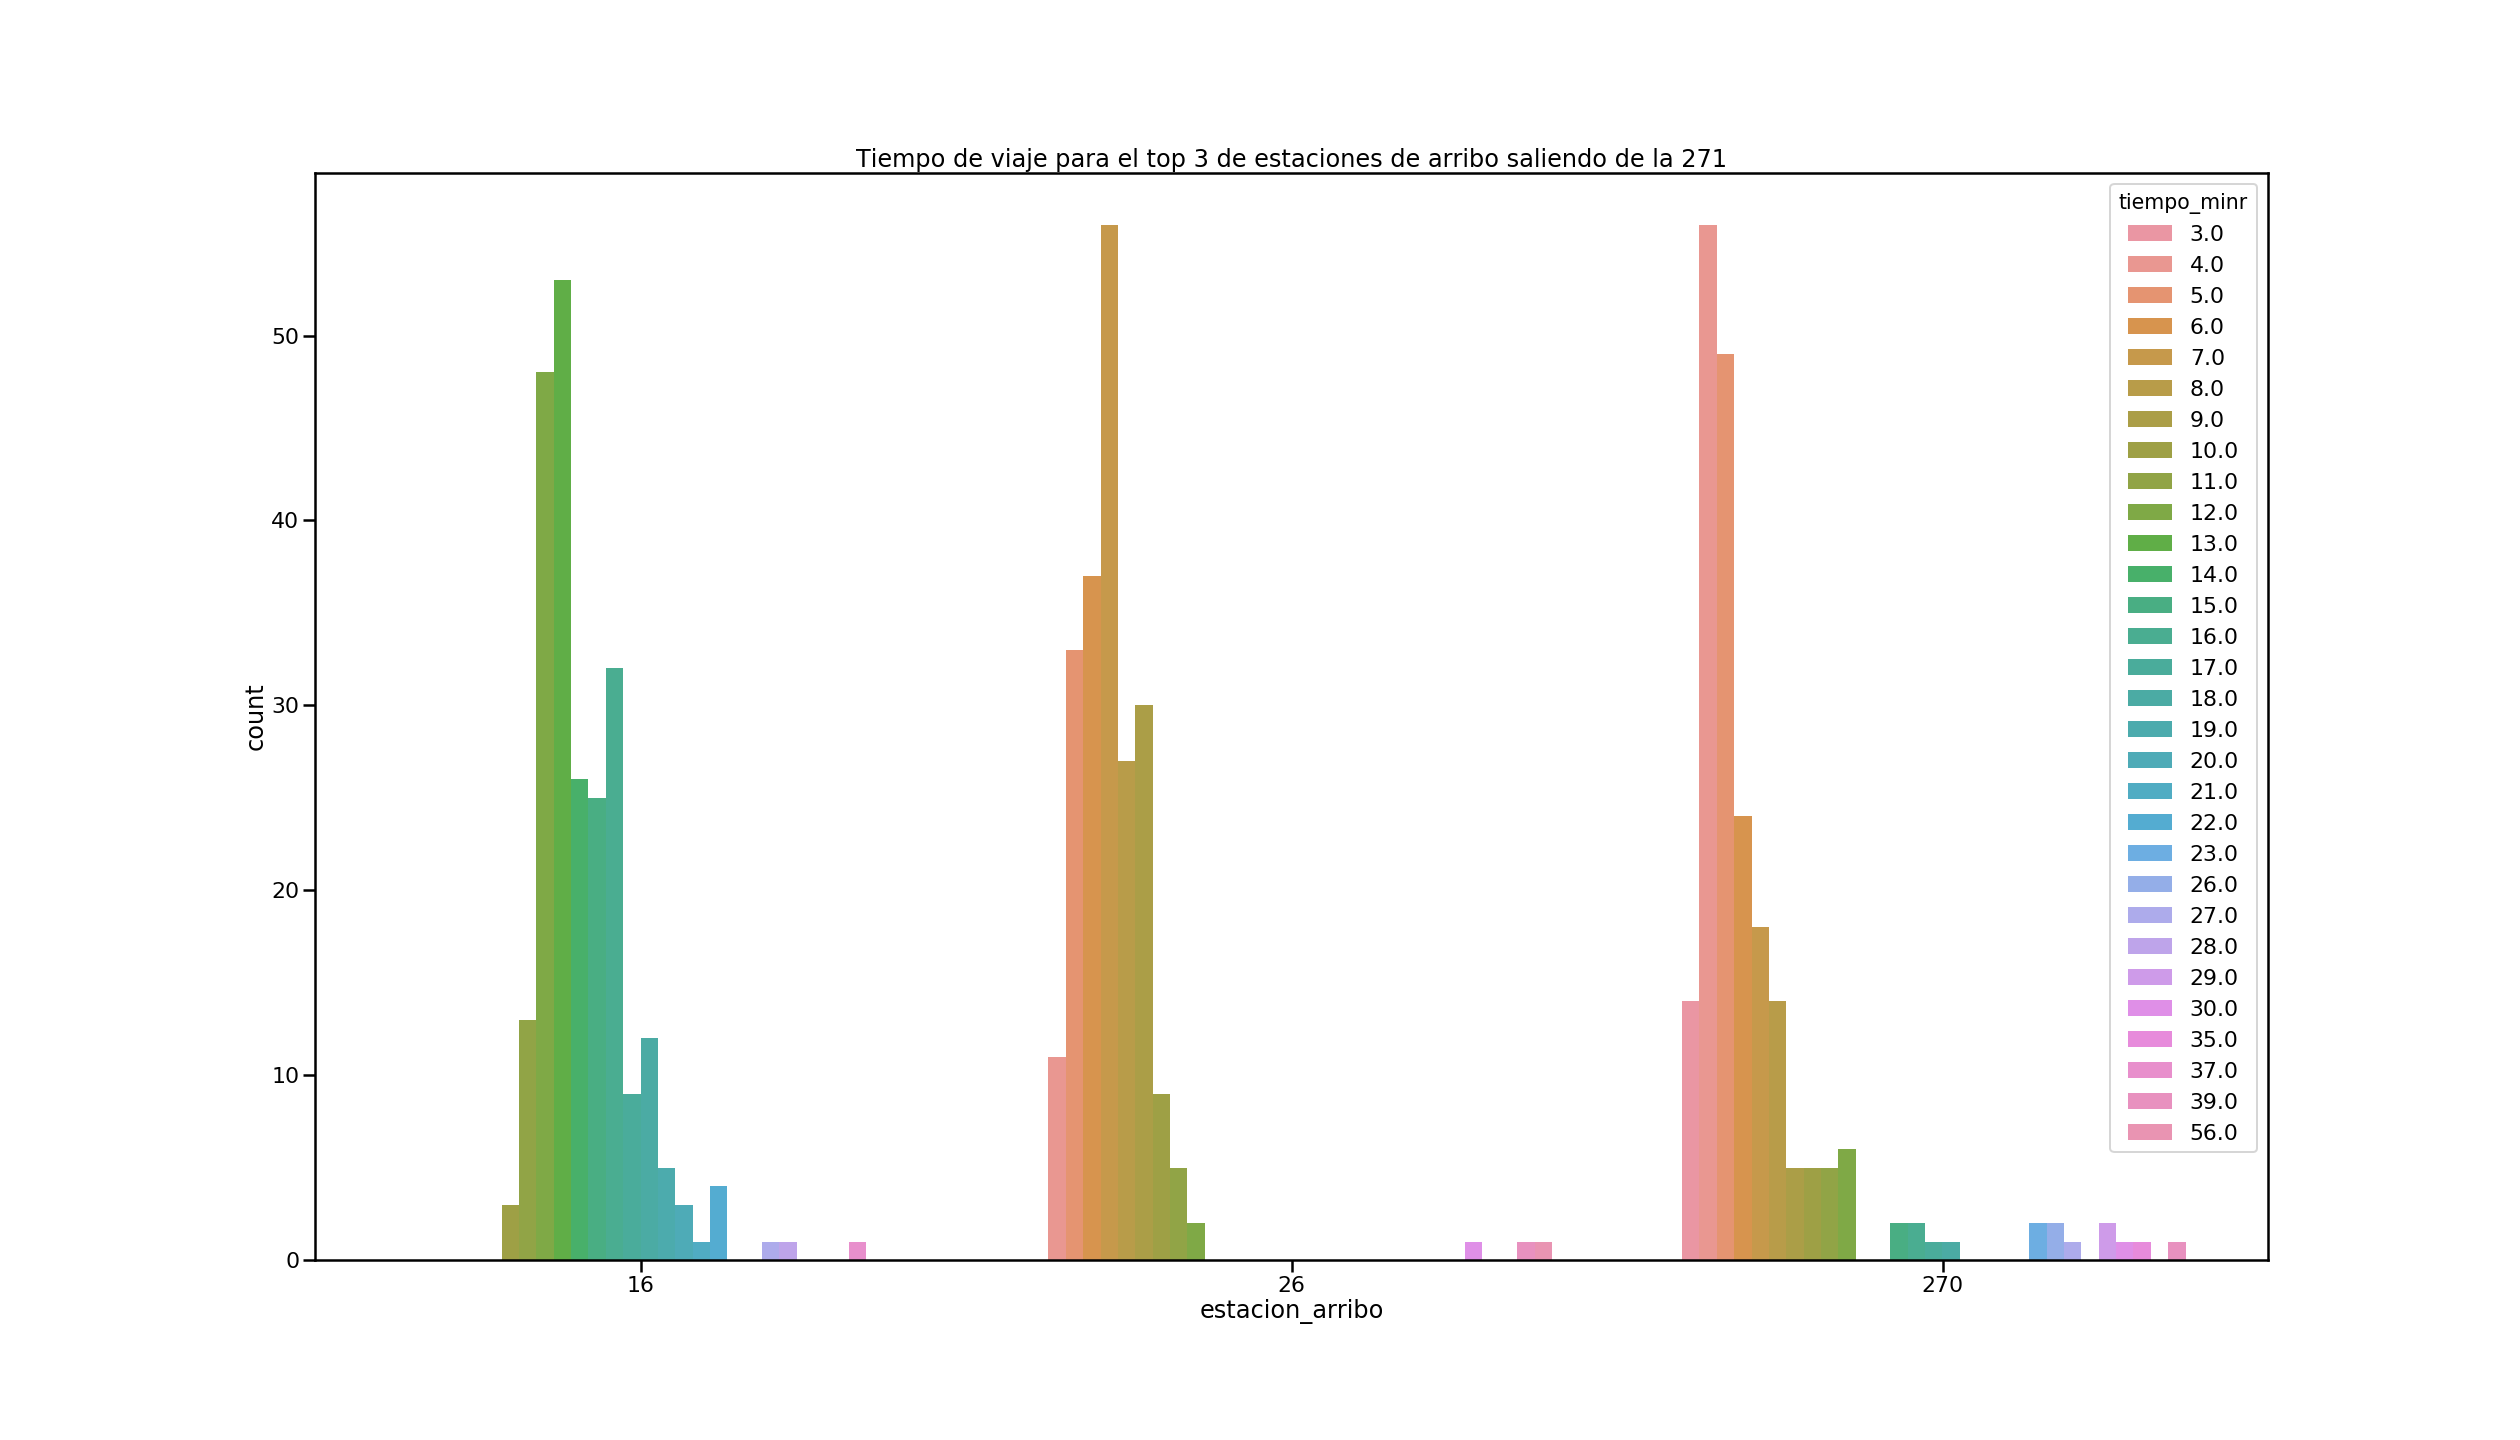
\includegraphics[width=0.9\linewidth]{Paper/images/tiempo_estaciones_271.png}
	\caption{ Tiempos de viaje al top 3 de estaciones de arribo para la estación 271}
	\label{fig:pen_habs_penbcestaciones}
\end{figure}
\begin{figure}[tbhp]
	\centering
	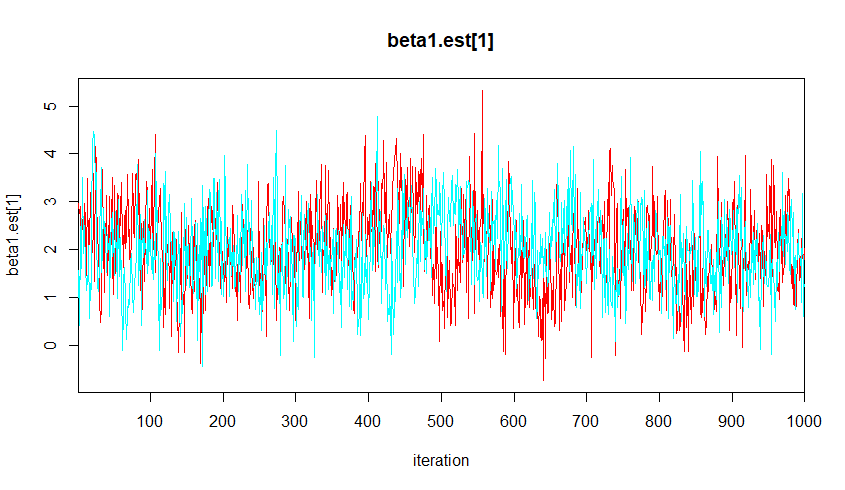
\includegraphics[width=0.9\linewidth]{Paper/images/303_cadenas_genero_1mujer.png}
	\caption{ Cicloestación 303 - convergencia de cadenas simuladas para género femenino}
	\label{fig:72_cadenas_femenino}
\end{figure}
\begin{figure}[tbhp]
	\centering
	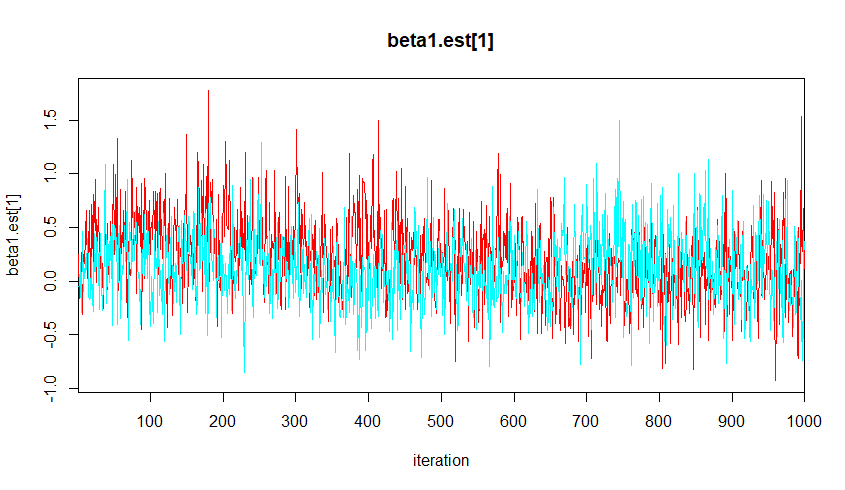
\includegraphics[width=0.9\linewidth]{Paper/images/72_cadenas_genero_1mujer.png}
	\caption{ Cicloestación 72 - convergencia de cadenas simuladas para género femenino}
	\label{fig:72_cadenas_femenino}
\end{figure}
\begin{figure}[tbhp]
	\centering
	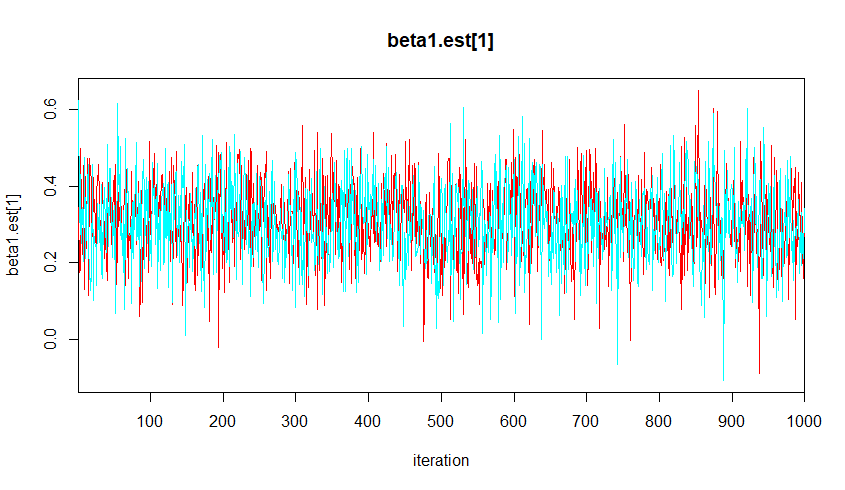
\includegraphics[width=0.9\linewidth]{Paper/images/271_cadenas_genero_1mujer.png}
	\caption{ Cicloestación 271 - convergencia de cadenas simuladas para género femenino}
	\label{fig:271_cadenas_femenino}
\end{figure}
\begin{figure}[tbhp]
	\centering
	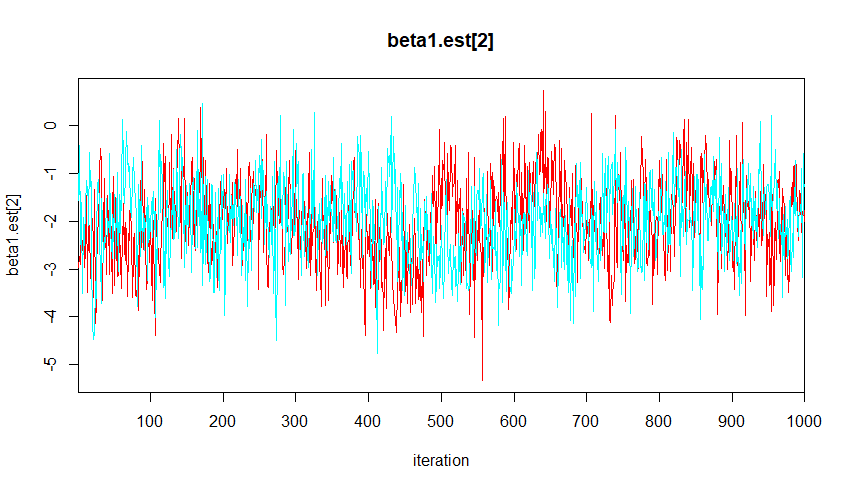
\includegraphics[width=0.9\linewidth]{Paper/images/303_cadenas_genero_2hombre.png}
	\caption{ Cicloestación 303 - convergencia de cadenas simuladas para género masculino}
	\label{fig:303_cadenas_masculino}
\end{figure}
\begin{figure}[tbhp]
	\centering
	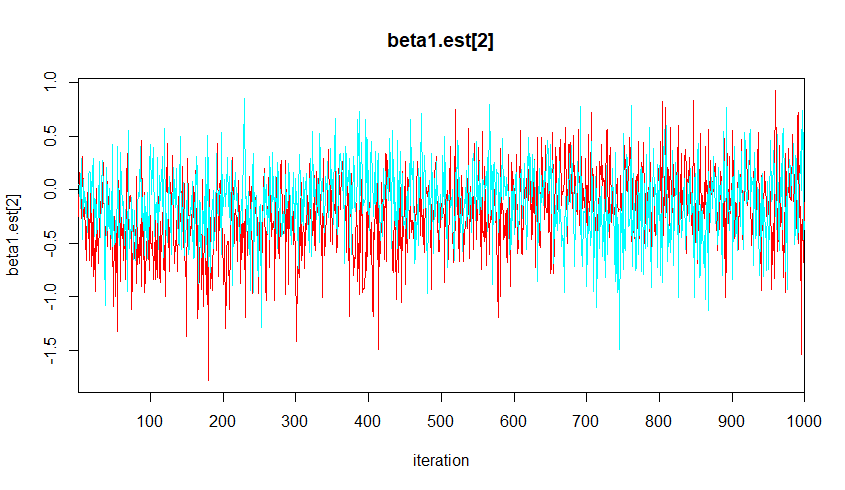
\includegraphics[width=0.9\linewidth]{Paper/images/72_cadenas_genero_2hombre.png}
	\caption{ Cicloestación 72 - convergencia de cadenas simuladas para género masculino}
	\label{fig:72_cadenas_masculino}
\end{figure}
\begin{figure}[tbhp]
	\centering
	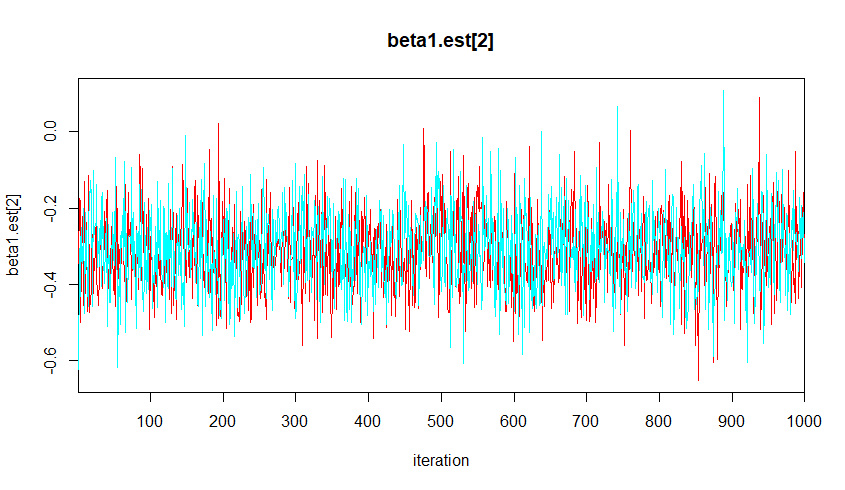
\includegraphics[width=0.9\linewidth]{Paper/images/271_cadenas_genero_2hombre.png}
	\caption{ Cicloestación 271 - convergencia de cadenas simuladas para género masculino}
	\label{fig:271_cadenas_masculino}
\end{figure}
\begin{figure}[tbhp]
	\centering
	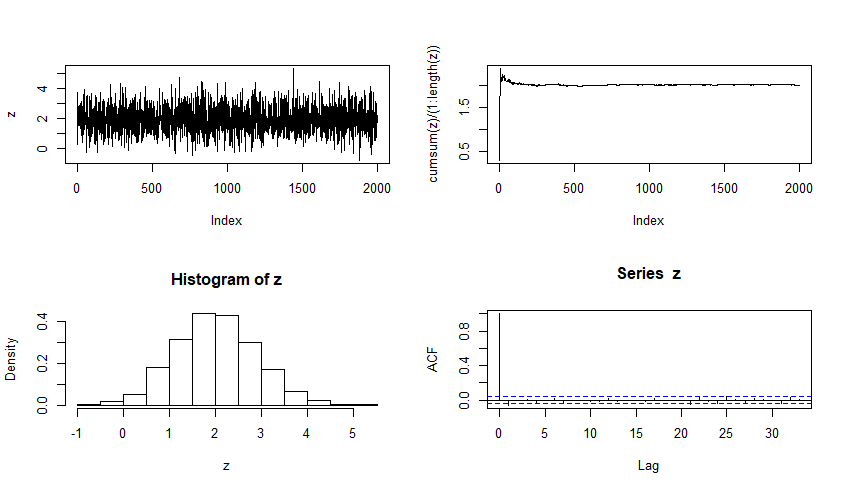
\includegraphics[width=0.9\linewidth]{Paper/images/303_genero_1mujer.png}
	\caption{ Cicloestación 303 - traceplot, promedios ergódicos, histograma de simulaciones y ACF para género femenino}
	\label{fig:303_traceplot_femenino}
\end{figure}
\begin{figure}[tbhp]
	\centering
	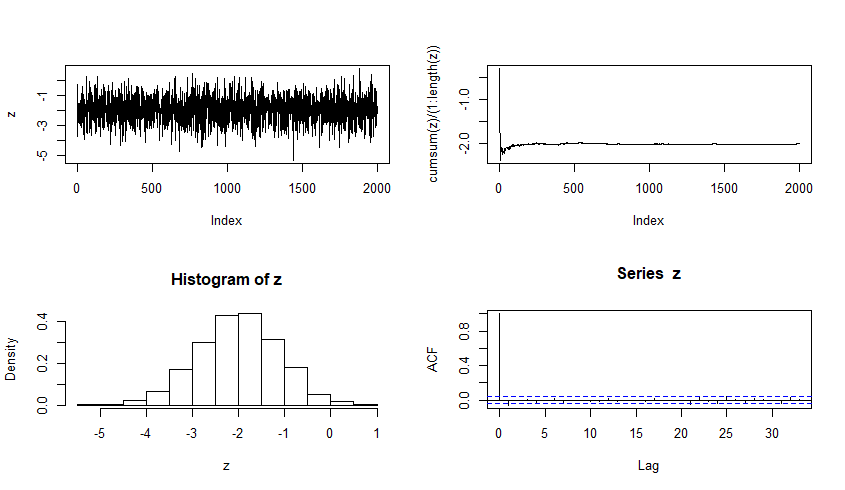
\includegraphics[width=0.9\linewidth]{Paper/images/303_genero_2hombre.png}
	\caption{ Cicloestación 303 - traceplot, promedios ergódicos, histograma de simulaciones y ACF para género masculino}
	\label{fig:303_traceplot_masculino}
\end{figure}
\begin{figure}[tbhp]
	\centering
	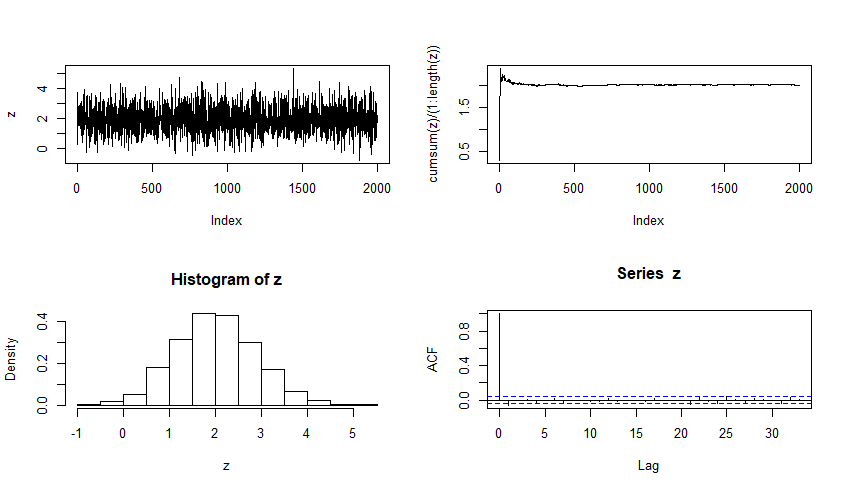
\includegraphics[width=0.9\linewidth]{Paper/images/72_genero_1mujer.png}
	\caption{ Cicloestación 72 -traceplot, promedios ergódicos, histograma de simulaciones y ACF para género femenino}
	\label{fig:72_traceplot_femenino}
\end{figure}
\begin{figure}[tbhp]
	\centering
	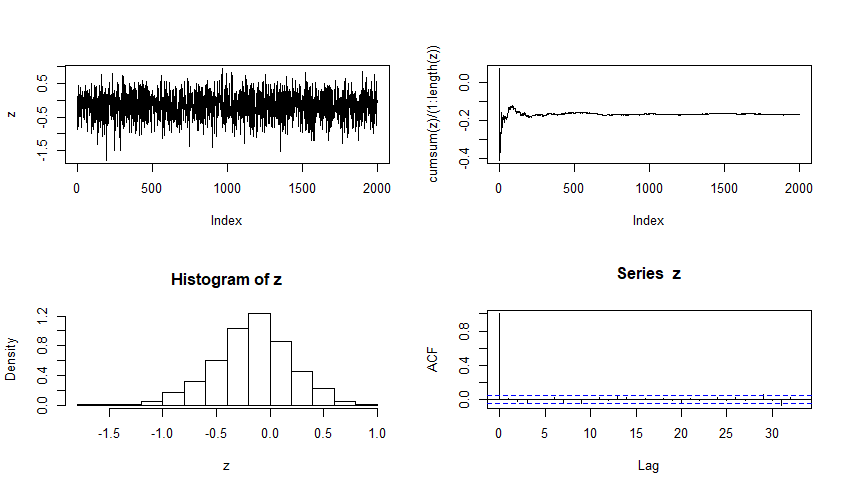
\includegraphics[width=0.9\linewidth]{Paper/images/72_genero_2hombre.png}
	\caption{ Cicloestación 72 - traceplot, promedios ergódicos, histograma de simulaciones y ACF para género masculino}
	\label{fig:72_traceplot_masculino}
\end{figure}

\begin{figure}[tbhp]
	\centering
	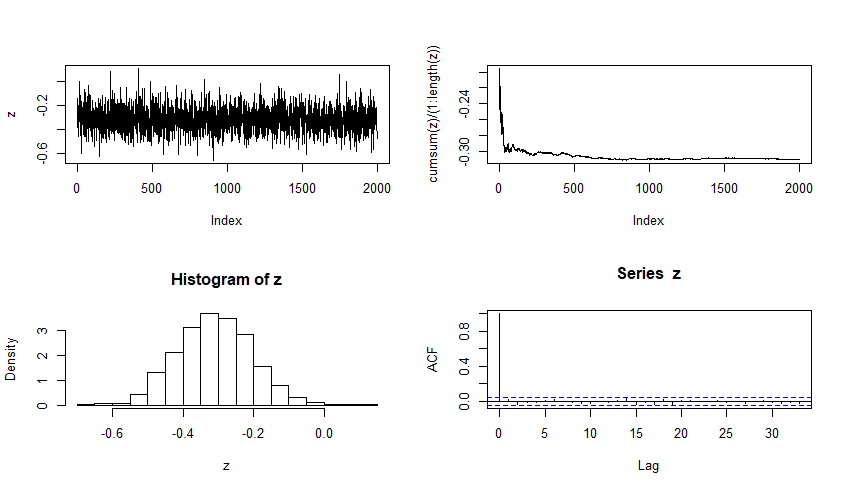
\includegraphics[width=0.9\linewidth]{Paper/images/271_genero_2hombre.png}
	\caption{ Cicloestación 271 -traceplot, promedios ergódicos, histograma de simulaciones y ACF para género masculino}
	\label{fig:pen_habs_penbc271_hombre}
\end{figure}

\begin{figure}[tbhp]
	\centering
	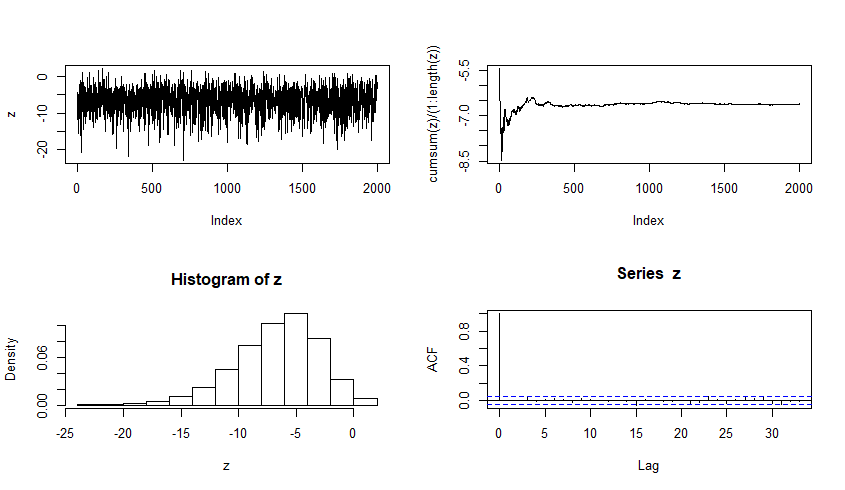
\includegraphics[width=0.9\linewidth]{Paper/images/303_diahora_7_21.png}
	\caption{ Cicloestación 303 - traceplot, promedios ergódicos, histograma de simulaciones y ACF para lunes 21 horas}
	\label{fig:pen_habs_penbc303_diahora}
\end{figure}
\begin{figure}[tbhp]
	\centering
	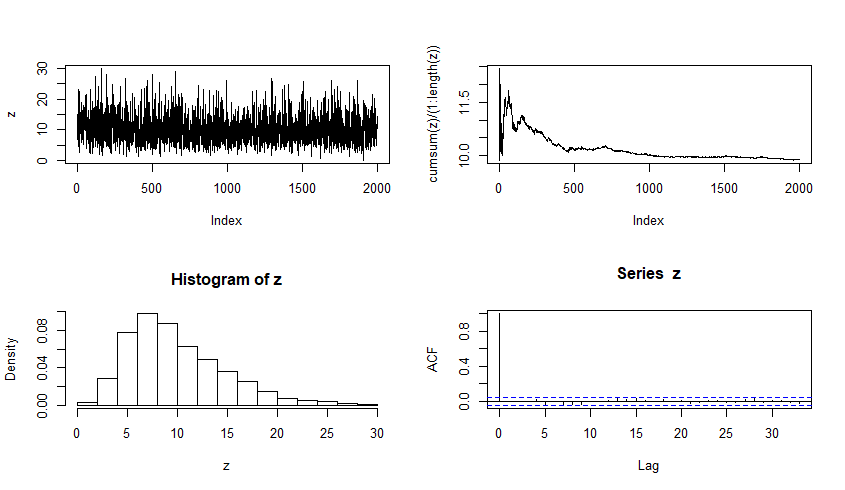
\includegraphics[width=0.9\linewidth]{Paper/images/72_diahora_7_21.png}
	\caption{ Cicloestación 72 -traceplot, promedios ergódicos, histograma de simulaciones y ACF para lunes 21 horas}
	\label{fig:pen_habs_penb72_diahora}
\end{figure}
\begin{figure}[tbhp]
	\centering
	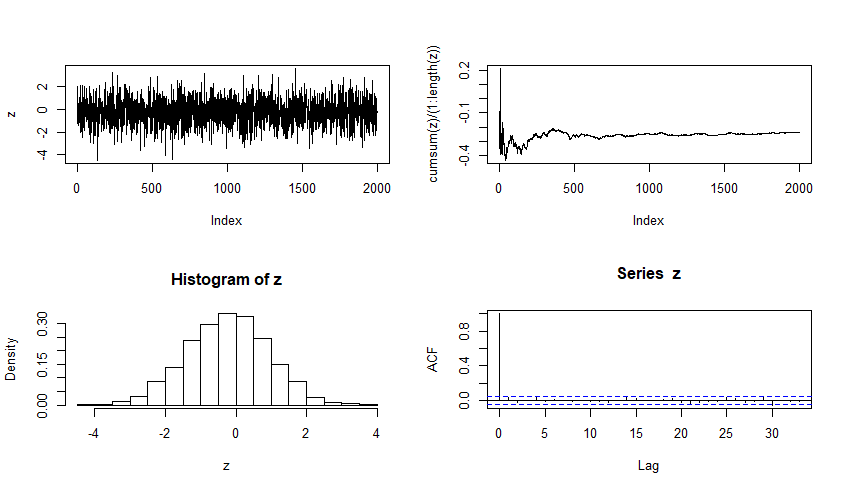
\includegraphics[width=0.9\linewidth]{Paper/images/271_diahora_7_21.png}
	\caption{ Cicloestación 271 - traceplot, promedios ergódicos, histograma de simulaciones y ACF para lunes 21 horas}
	\label{fig:pen_habs_penbces271_diahora}
\end{figure}
\begin{figure}[tbhp]
	\centering
	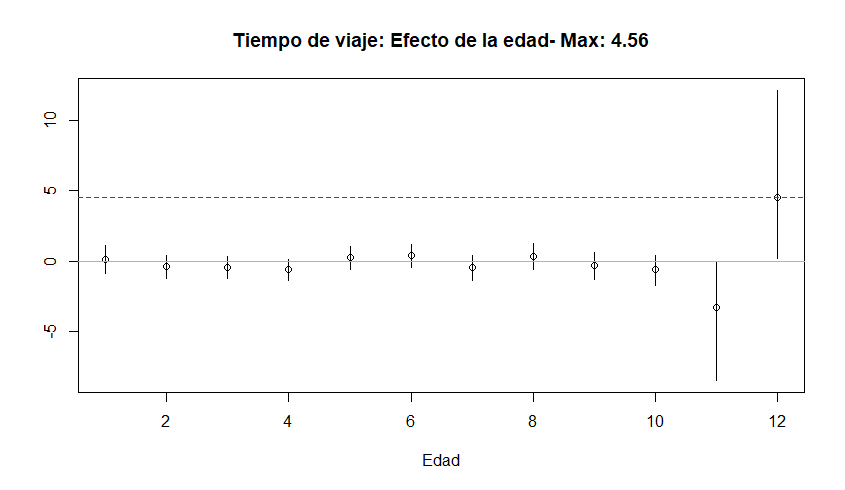
\includegraphics[width=0.9\linewidth]{Paper/images/72_efecto_edad.png}
	\caption{ Efecto del grupo de edad en la duración del viaje}
	\label{fig:72_efecto_edad}
\end{figure}
\end{appendices}
\end{document}
